\chapter*{Perusahaan Dunia yang menggunakan bahasa pemrograman Python}

\section*{\textit{Spotify}}
\par
\textit{Spotify} adalah suatu layanan musik streaming yang memanfaatkan bahasa pemprograman python untuk analisis data dan backend. Pada backend spotify berkomunikasi dengan 0MQ. 0MQ itu sendiri adalah suatu framework dan library open source untuk networking. Untuk menginterpretasikan analisis data tersebut spotify menggunakan luigi, dan modul python yang sinkron dengan hadoop. Modul open source ini menangani satu library dengan library lainnya agar saling bekerjasama, serta dapat mengkonsolidasi eror log secara cepat.
\section*{\textit{Google}}
\par
\textit{Google} ini sudah menggunakan bahasa pemprograman python ini sudah sajak dari awal berdirinya. Dan pada saat ini bahasa pemprograman python merupakan salah satu bahasa pemprograman server-side resmi di google. Meskipun ada script yang ditulis untuk google menggunakan bahasa perl dan bash, maka nantinya script tersebut akan diubah ke python terlebih dahulu, karena kemudahan dalam perawatannya.

\section*{\textit{Industrial Light and Magic}}
\par
\textit{Industrial Light and Magic} merupakan studio special efek yang dibutuhkan untuk film star wars saja. Karena infrastruktur awal industrial light and magisc ini menggunakan C dan C++, maka akan lebih mudah mengintegrasikan bahasa pemprograman python ketimbang bahasa pemprograman lainnya. Dengan menggunakan bahasa pemprogramana python ini industrial light and magic dengan mudah membungkus komponen software dan dapat meningkatkan aplikasi grafisnya.

\section*{\textit{Netflix}}
\par
\textit{Netflix} adalah suatu layanan pemutaran film yang dapat dilakukan oleh pengguna dimanapun dan kapanpun. Pada netfilx bahasa pemprograman yang digunakan adalah bahasa pemprograman python, bahasa pemprograman ini digunakan pada Central Alert Gateway yang akan me-reroute alert dan mengirimkannya pada individu yang akan melihatnya serta juga  dapat secara otomatis reboot atau menghentikan proses yang dianggap bermasalah. Selain itu python juga digunakan untuk menelusuri riwayat dan perubahan pengaturan keamanan.

\section*{\textit{Instagram}}
\textit{Instagram} adalah suatu aplikasi mobile berbasis IOS, android dan windows phone, dimana pengguna dapat berbagi foto dan video melalui instagram ini. Pada instagram ini menggunakan bahasa pemprograman python dalam task queuennya atau fitur dimana setiap pengguna dapat berbagi foto atau video ke beberapa social network lainnya seperti facebook, twitter, dan lain-lainnya.

Selain perusahaan diatas ada beberapa perusahaan pengguna Python lain yaitu: Pinterest, Disqus, Dropbox, Uber, Reddit, Quora, Facebook (Bahasa ke-3 setelah PHP (Hack) dan C++, digunakan untuk manajemen infrastruktur).
\par
\chapter*{CARA INSTALLER APLIKASI}
\section*{CARA INSTALLER ANACONDA} 
\begin{enumerate}
\item Pertama buka anaconda pada google, kemudian cari installer anaconda versi 3
    \begin{figure}[h]
    \centering
    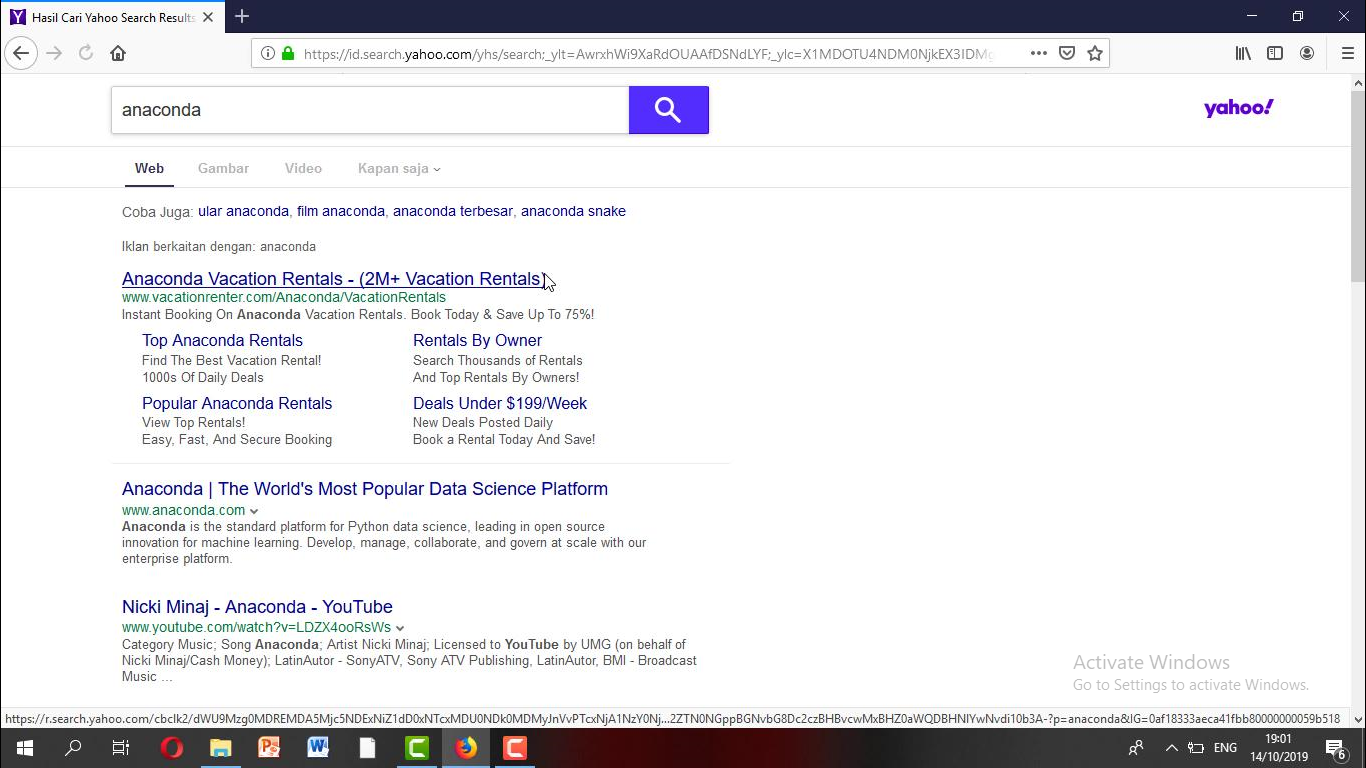
\includegraphics[scale=0.2]{gambar/1.png}
    \caption{}
    \label{fig:my_label}
\end{figure}
\item 	Selanjutnya klik download pada pojok kanan atas
\begin{figure}[h]
    \centering
    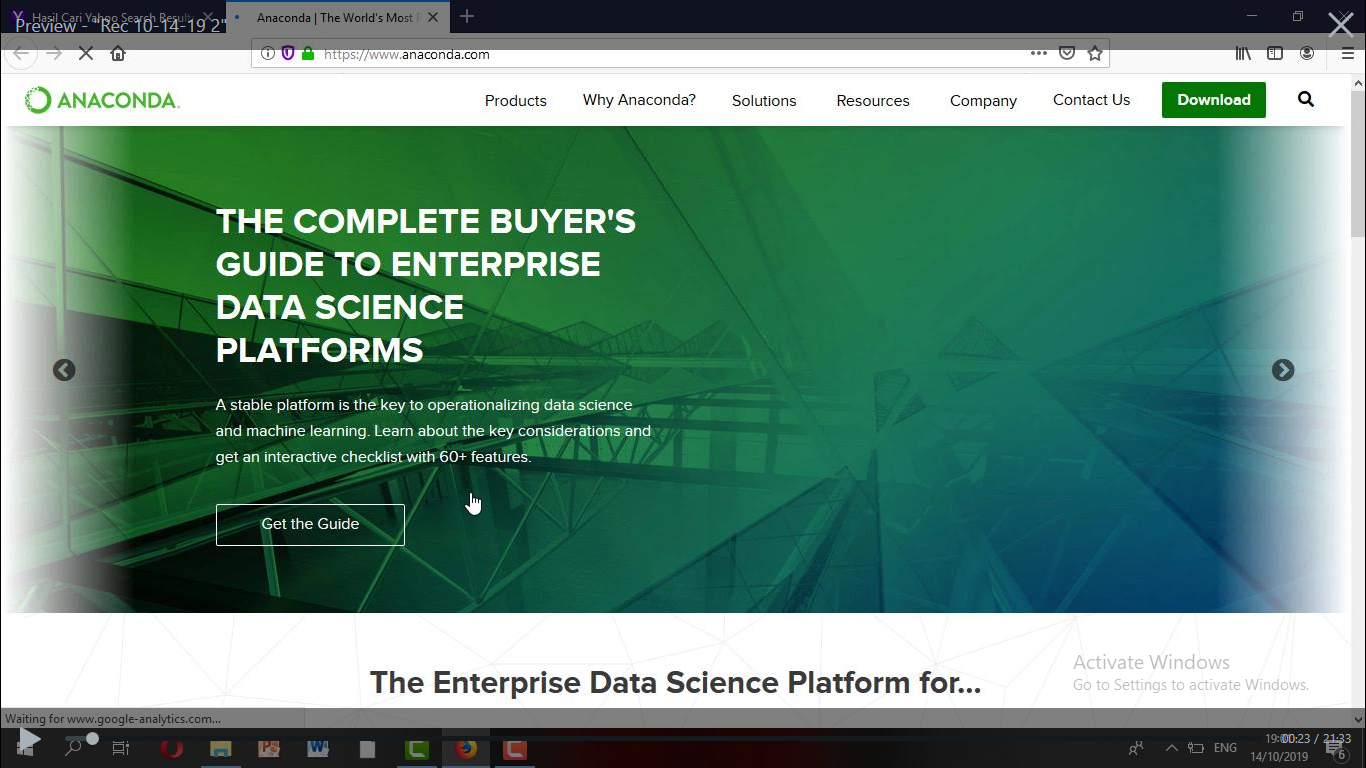
\includegraphics[scale=0.2]{gambar/2.png}
    \caption{}
    \label{fig:my_label}
\end{figure}
\item 	Kemudian pilih versi tergantung berapa bit laptop anda, kalau laptop anda 32 bit maka pakai yang 32 bit tapi jika laptop anda 64 bit maka pakailah yang 64 bit.
\begin{figure}[h]
    \centering
    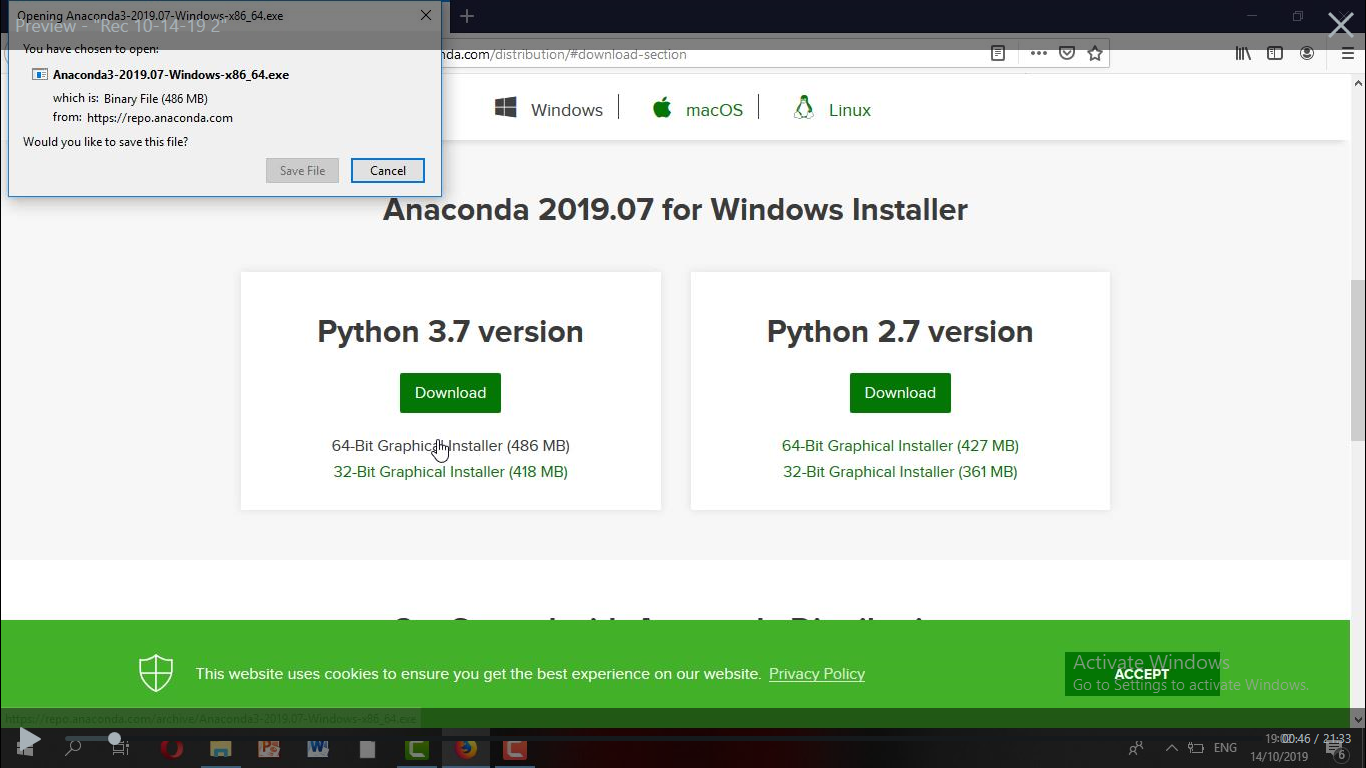
\includegraphics[scale=0.2]{gambar/3.png}
    \caption{}
    \label{fig:my_label}
\end{figure}
\item  Selanjutnya klik I agree
\begin{figure}[h]
    \centering
    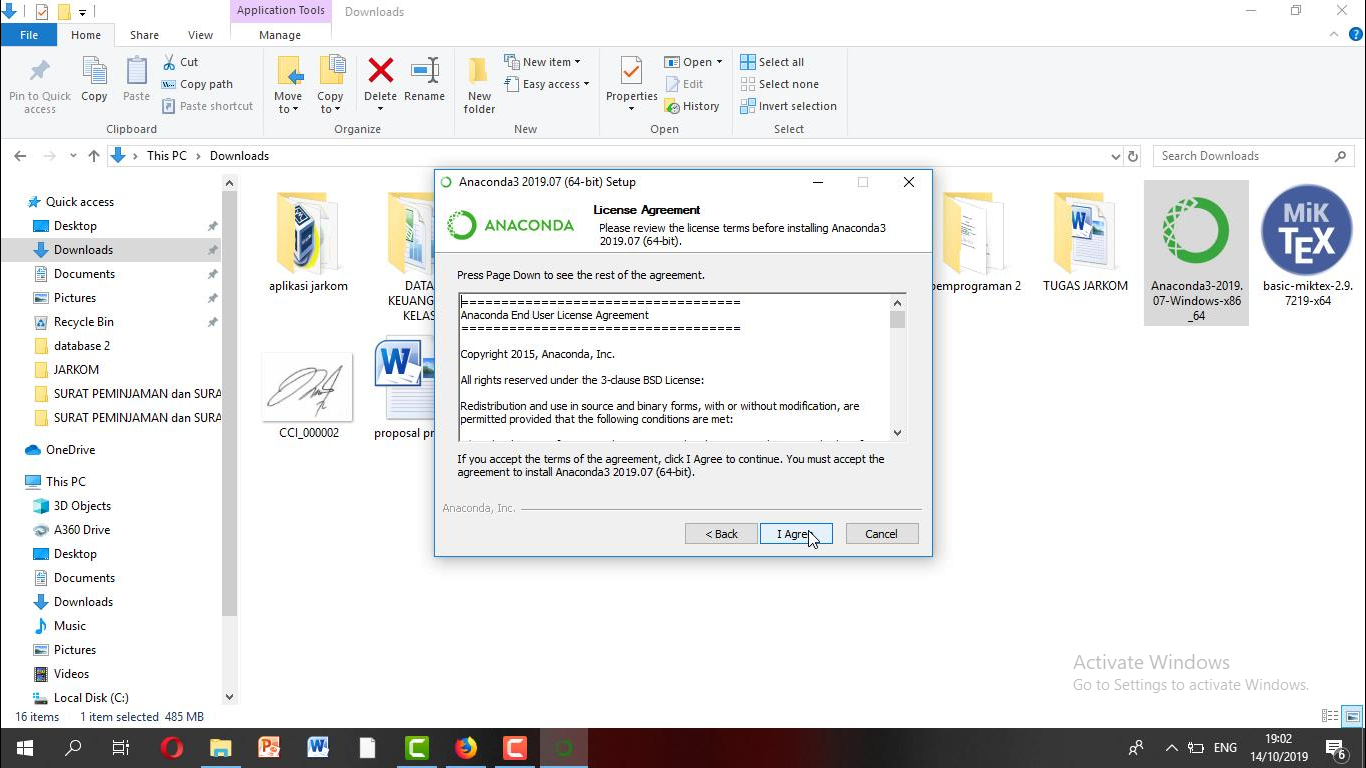
\includegraphics[scale=0.2]{gambar/4.png}
    \caption{}
    \label{fig:my_label}
\end{figure}
\item  Lalu klik next
\begin{figure}[h]
    \centering
    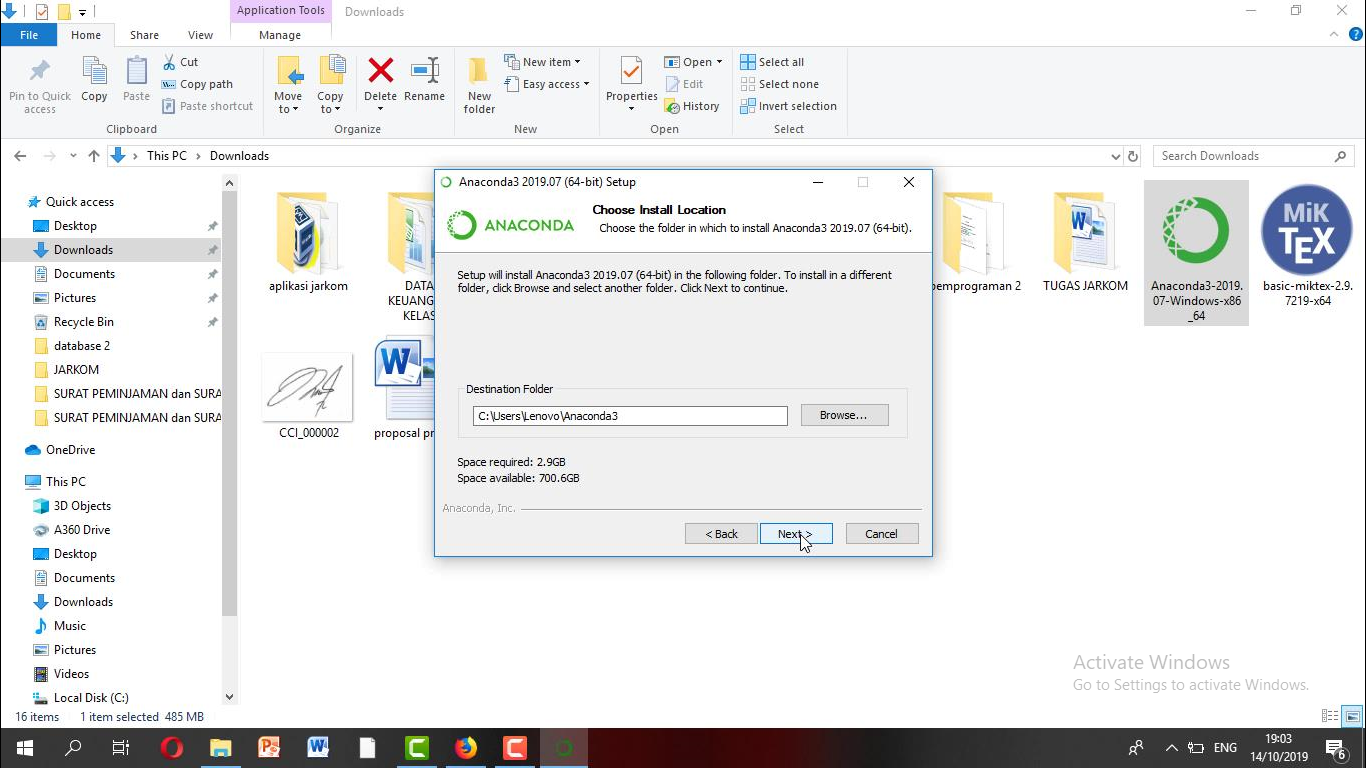
\includegraphics[scale=0.2]{gambar/5.png}
    \caption{}
    \label{fig:my_label}
\end{figure}
\item  Kemudian akan mucul kotak dialog dan centang kedua-duanya, lalu klik install.
\begin{figure}[h]
    \centering
    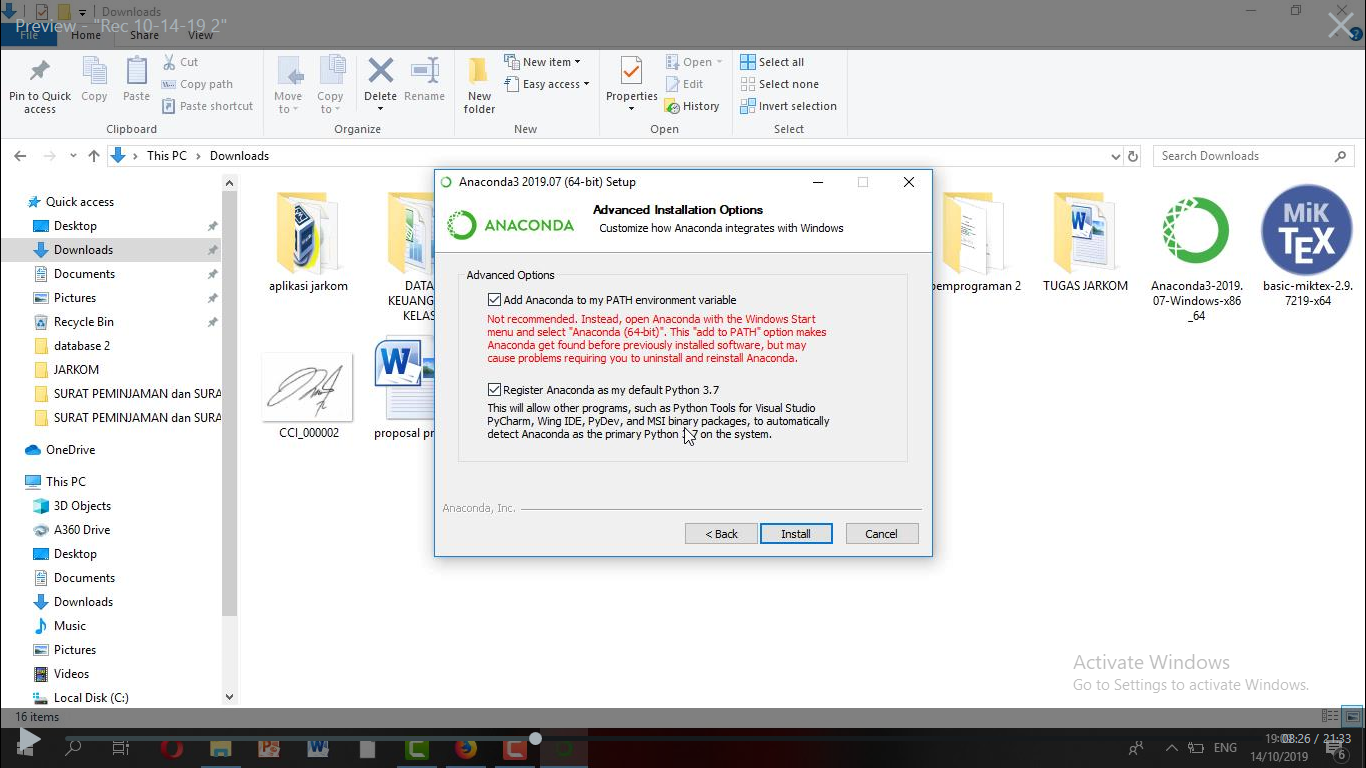
\includegraphics[scale=0.2]{gambar/6.png}
    \caption{}
    \label{fig:my_label}
\end{figure}
\item  Tunggu hingga proses install selesai
\begin{figure}[h]
    \centering
    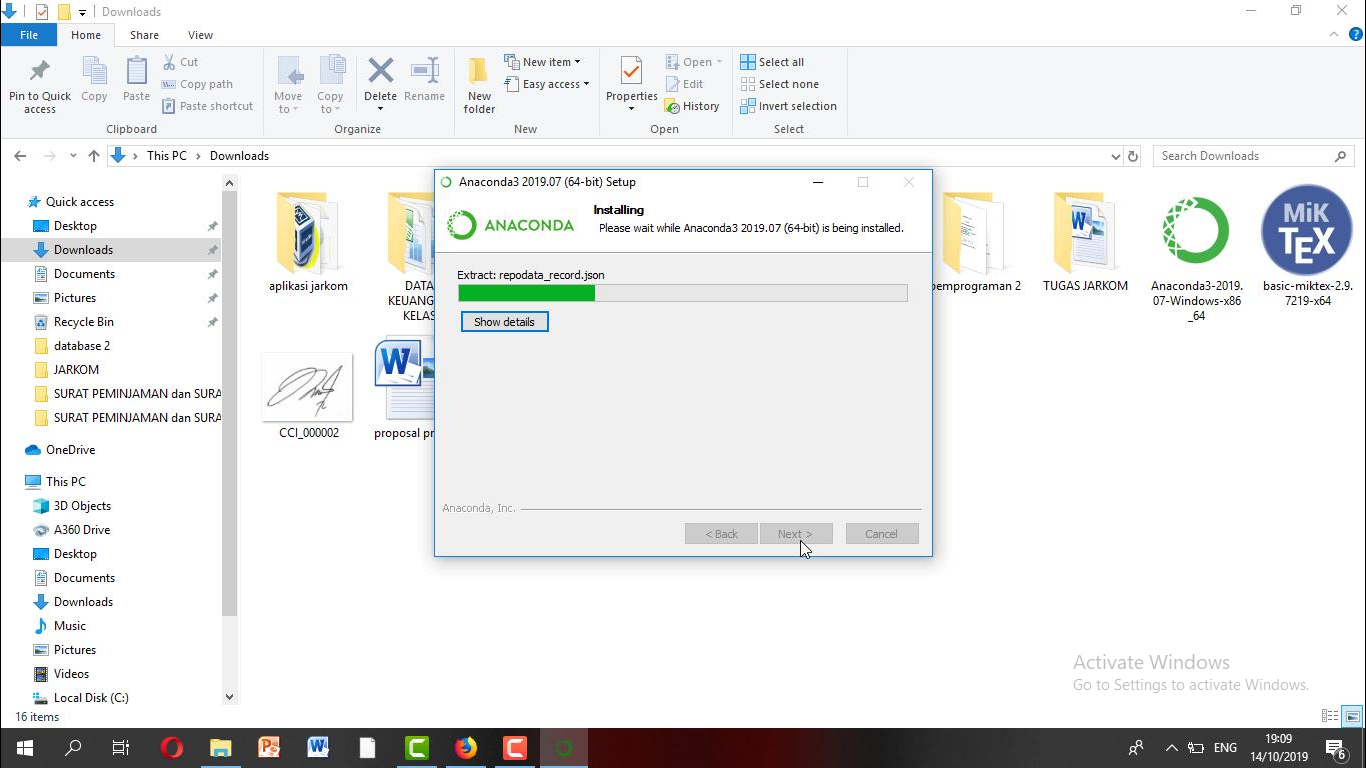
\includegraphics[scale=0.2]{gambar/7.png}
    \caption{}
    \label{fig:my_label}
\end{figure}
\item  Setelah itu klik next
\begin{figure}[h]
    \centering
    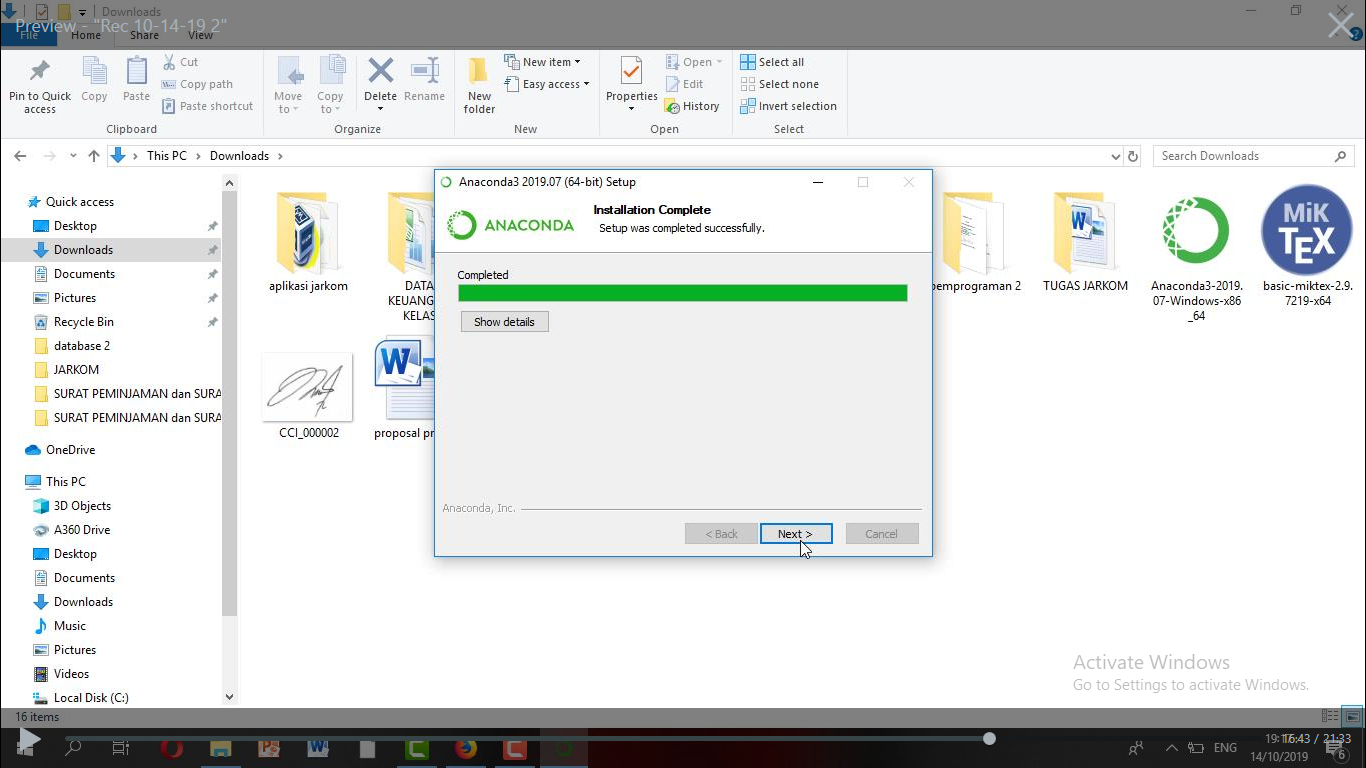
\includegraphics[scale=0.2]{gambar/8.png}
    \caption{}
    \label{fig:my_label}
\end{figure}
\item  Kemudian klik next lagi
\begin{figure}[h]
    \centering
    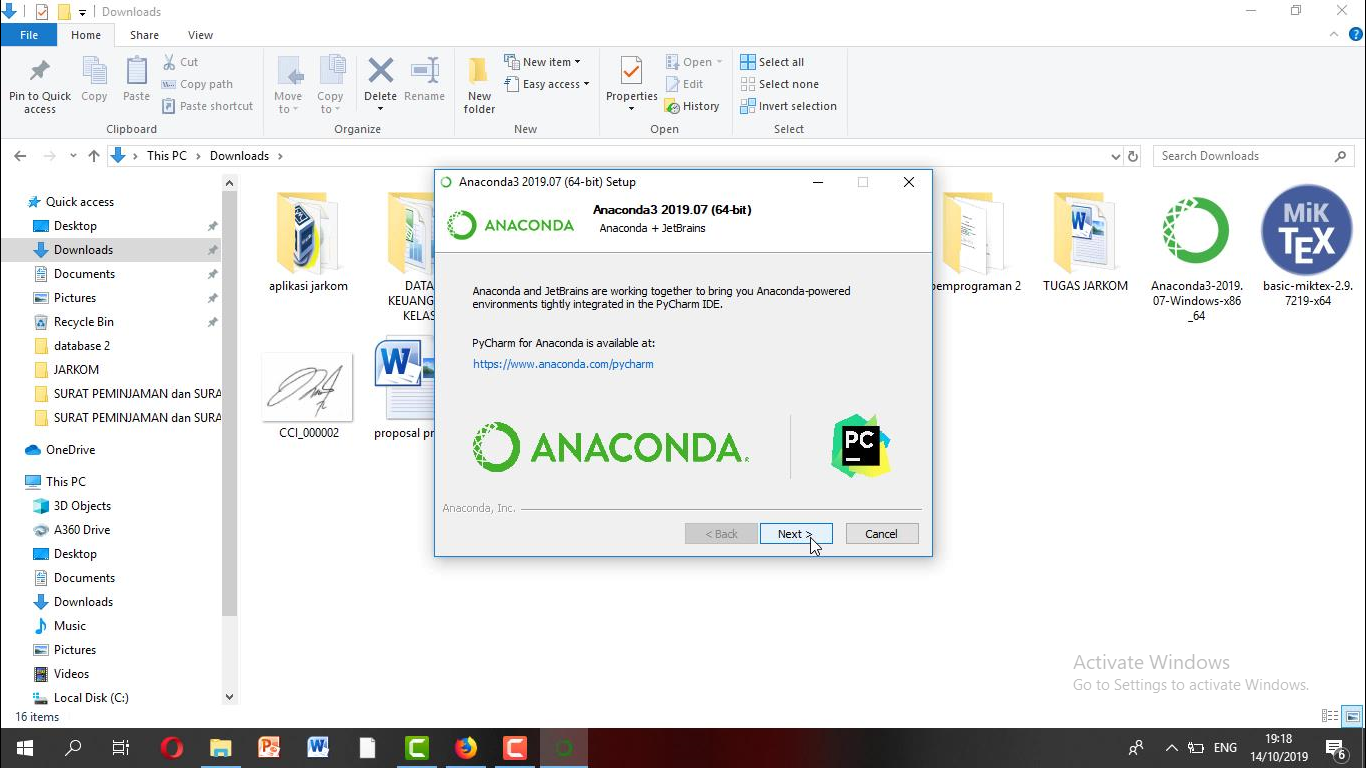
\includegraphics[scale=0.2]{gambar/9.png}
    \caption{}
    \label{fig:my_label}
\end{figure}
\item  Dan terakhir klik finish
\begin{figure}[h]
    \centering
    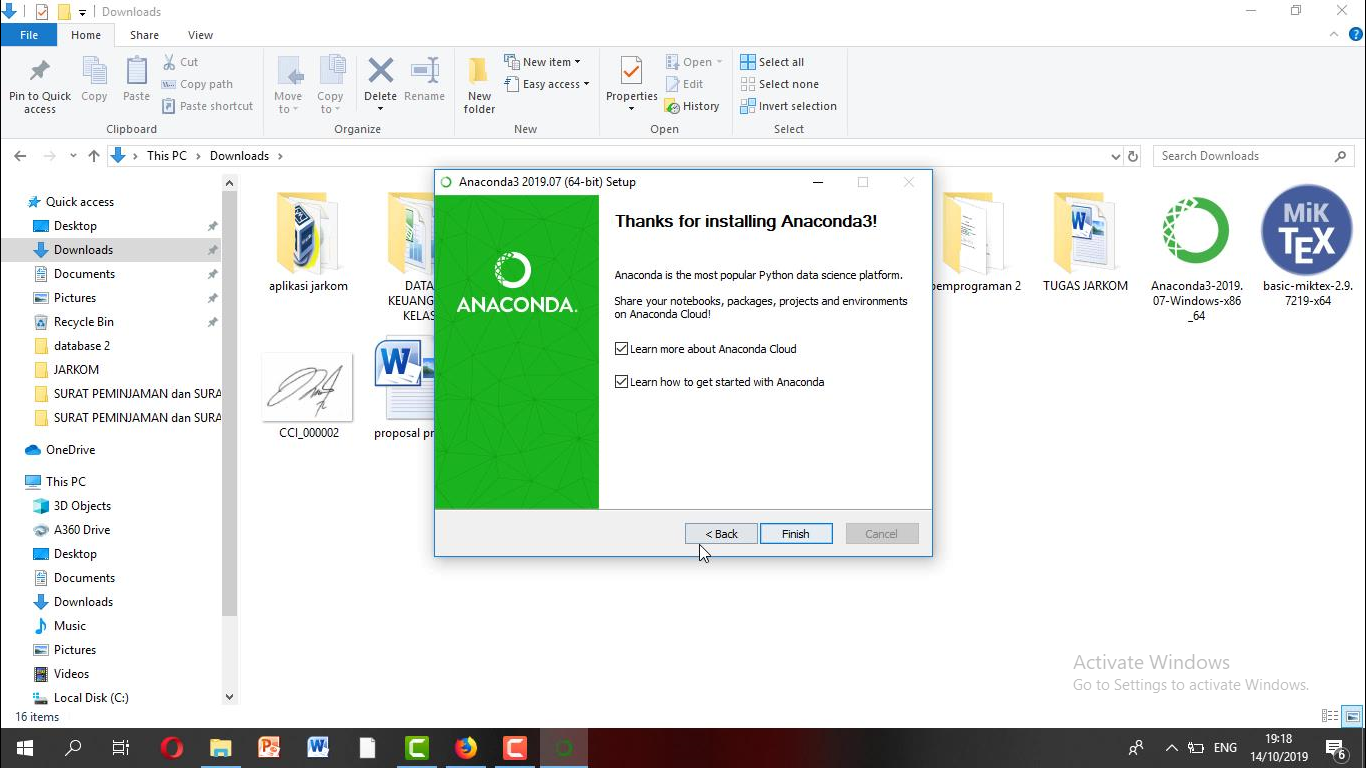
\includegraphics[scale=0.2]{gambar/10.png}
    \caption{}
    \label{fig:my_label}
\end{figure}
\section*{CARA INSTALLER PIP}
\begin{enumerate}
\item  Caranya agak mirip dengan install python, yaitu pertama searching pip pada google.
\begin{figure}[h]
    \centering
    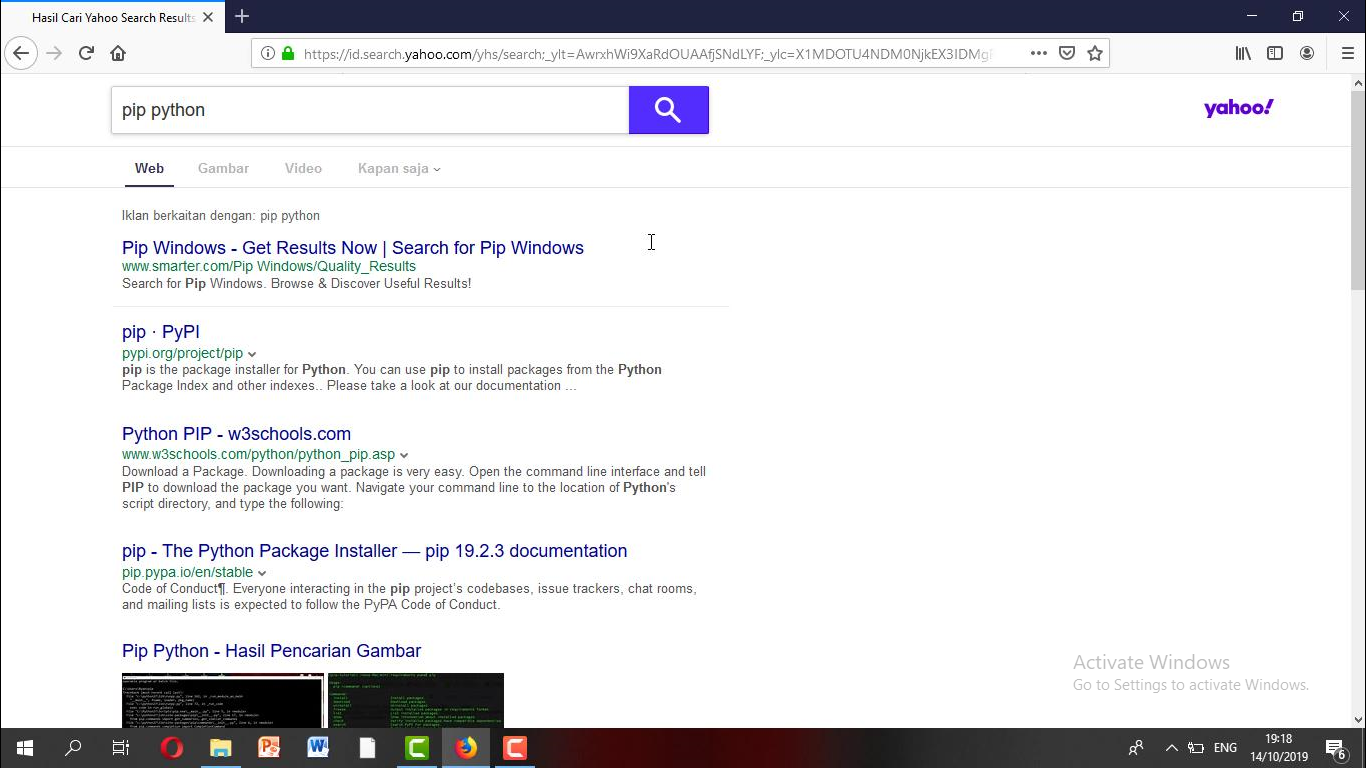
\includegraphics[scale=0.2]{gambar/11.png}
    \caption{}
    \label{fig:my_label}
\end{figure}
\item  Lalu klik installation,seperti yang ditunjuk tanda panah
\begin{figure}[h]
    \centering
    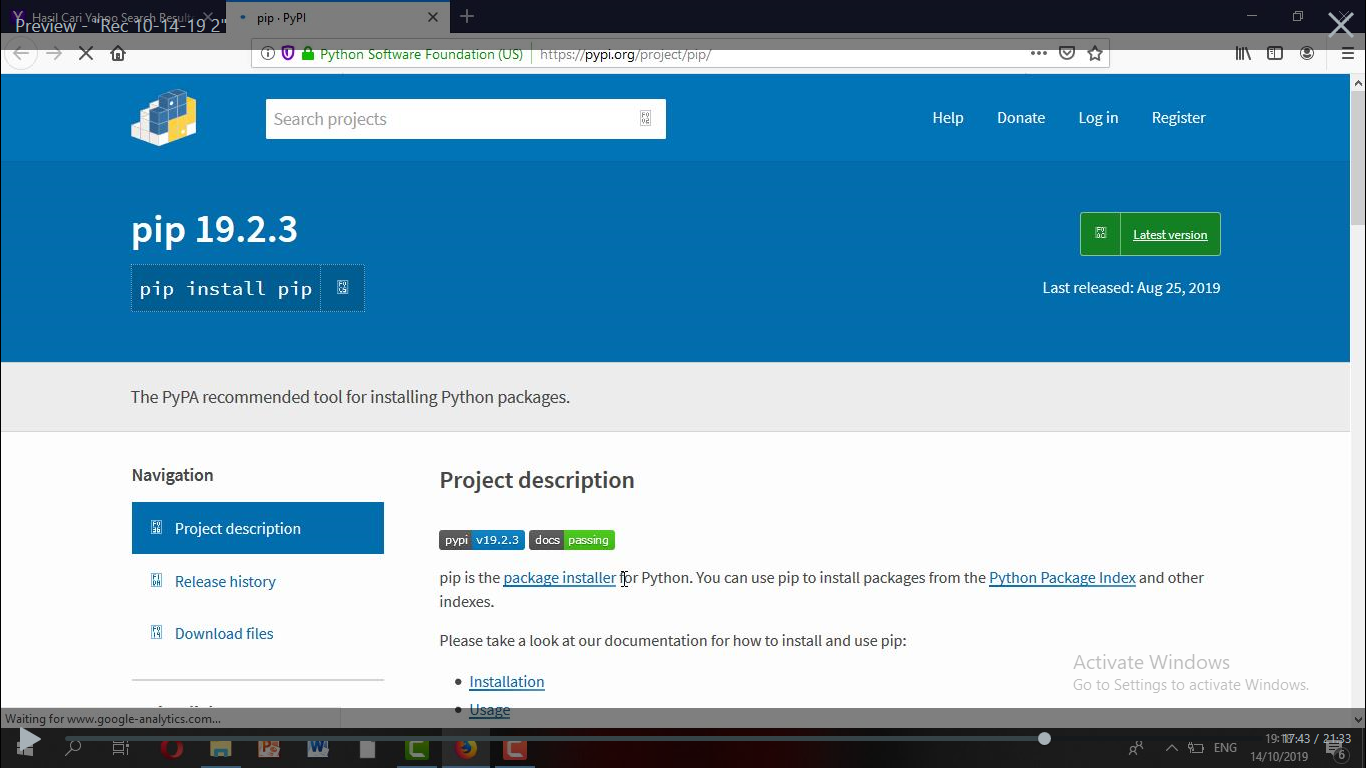
\includegraphics[scale=0.2]{gambar/12.png}
    \caption{}
    \label{fig:my_label}
\end{figure}
\item  Kemudian klik get.pip.py seperti yang ditunjuk tanda panah dibawah ini, lalu klik ok.
\begin{figure}[h]
    \centering
    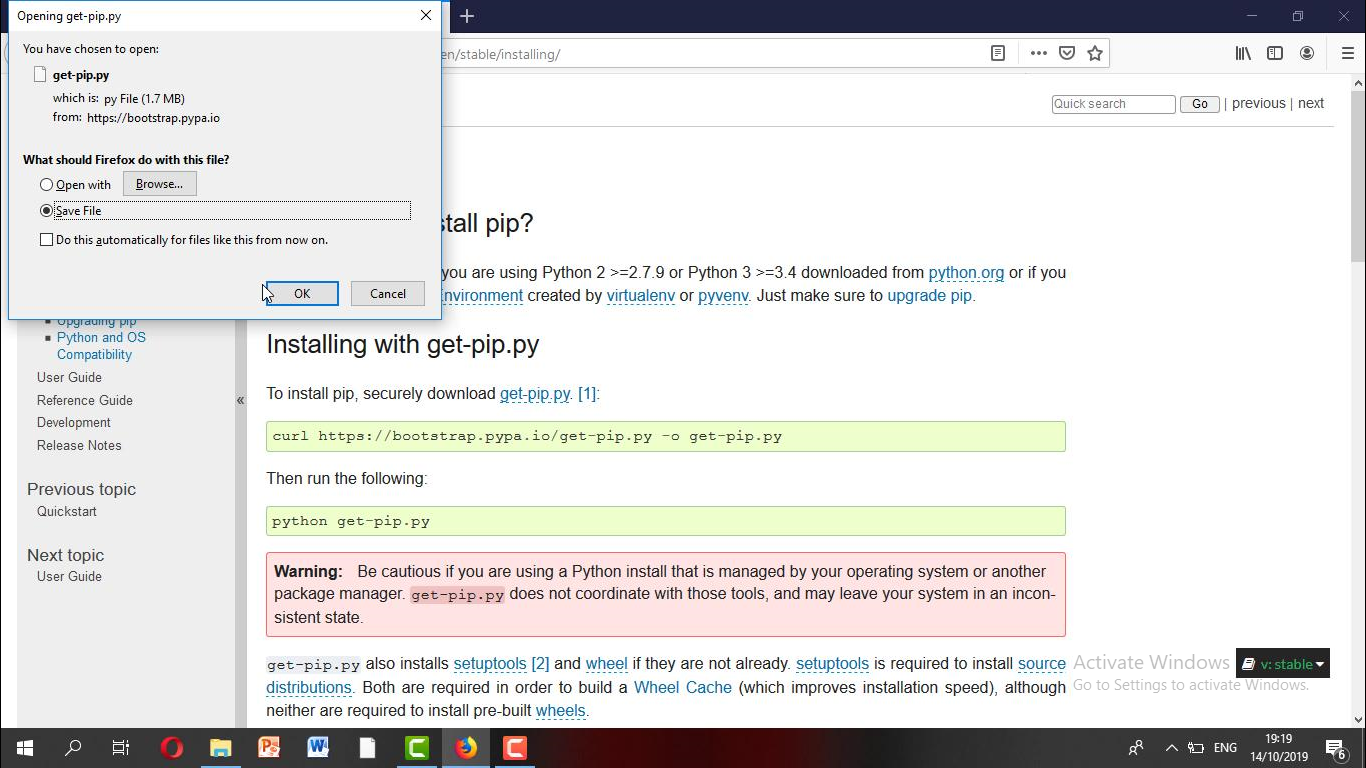
\includegraphics[scale=0.2]{gambar/13.png}
    \caption{}
    \label{fig:my_label}
\end{figure}
\item  Setelah itu buka cmd
\begin{figure}[h]
    \centering
    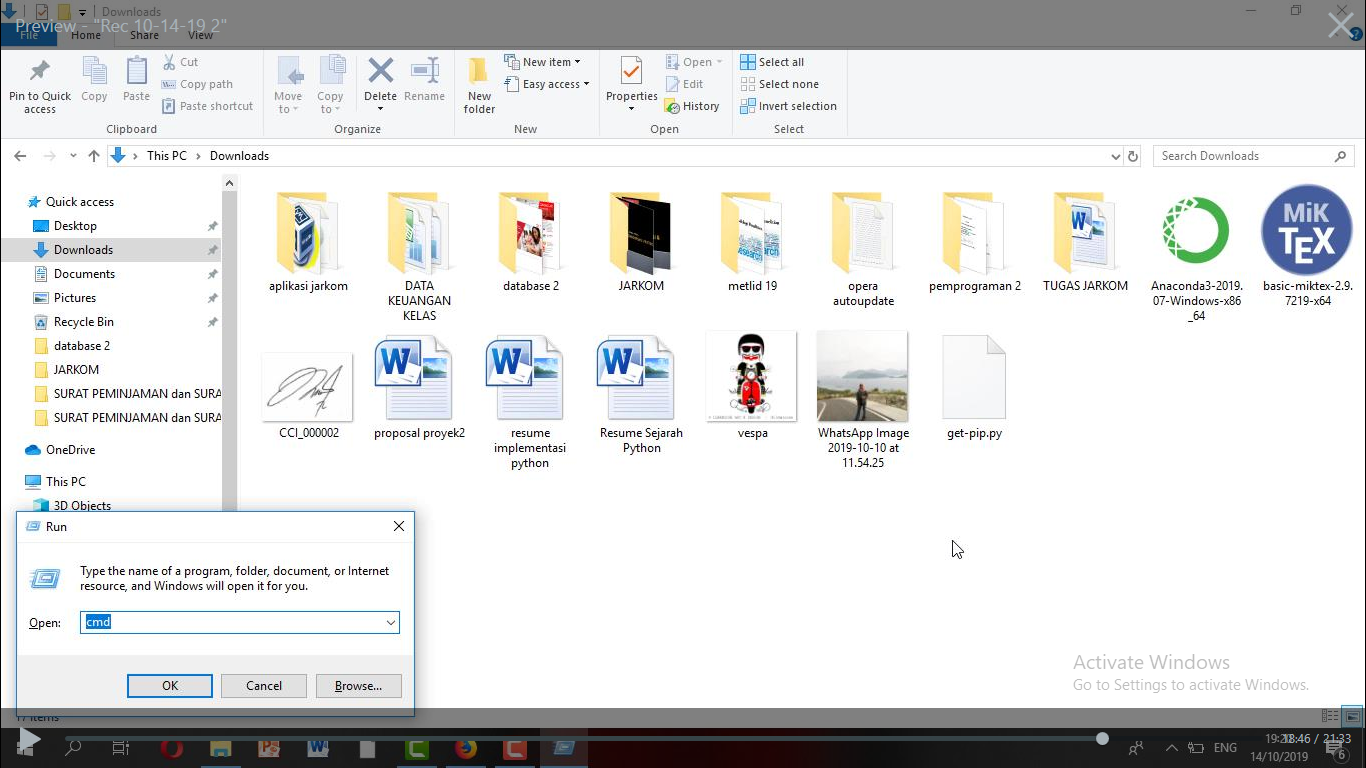
\includegraphics[scale=0.2]{gambar/14.png}
    \caption{}
    \label{fig:my_label}
\end{figure}
\item  Lalu ketik  python get.pip.py
\begin{figure}[h]
    \centering
    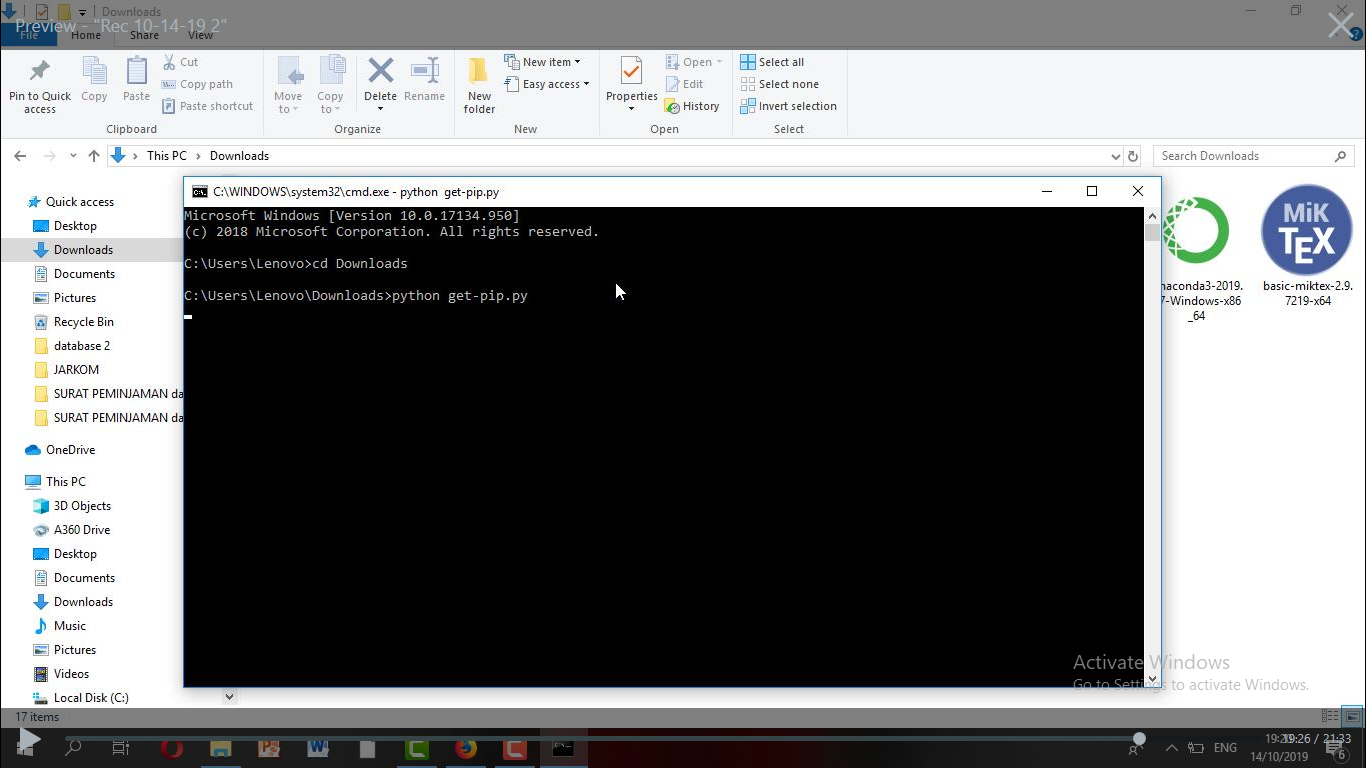
\includegraphics[scale=0.2]{gambar/15.png}
    \caption{}
    \label{fig:my_label}
\end{figure}
\item Jika tampilanya sudah seperti gambar yang dibawah ini, maka sudah selesai.
\begin{figure}[h]
    \centering
    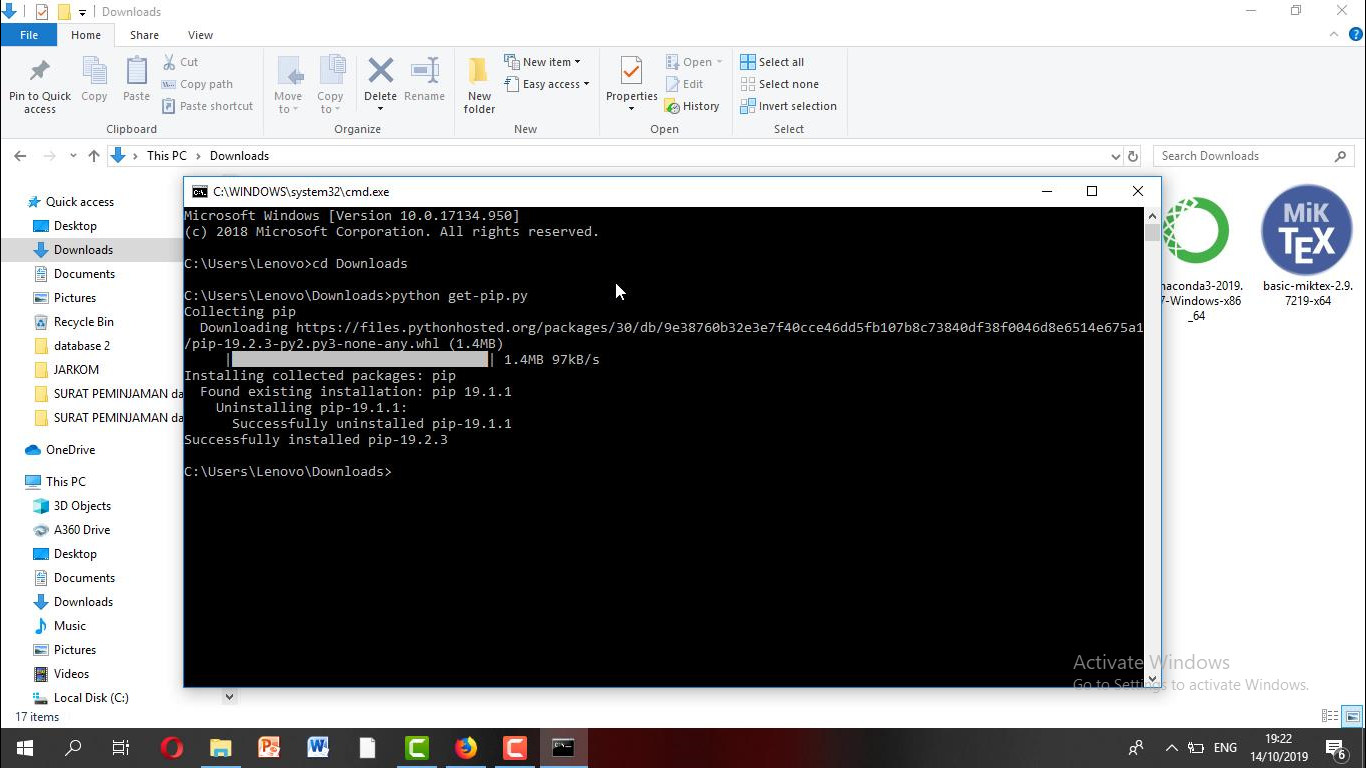
\includegraphics[scale=0.2]{gambar/16.png}
    \caption{}
    \label{fig:my_label}
\end{figure}
\section*{CARA UPDATE SPYDER DAN ANACONDA}
\begin{enumerate}
\item Pertama buka aplikasi anacondanya
\begin{figure}[h]
    \centering
    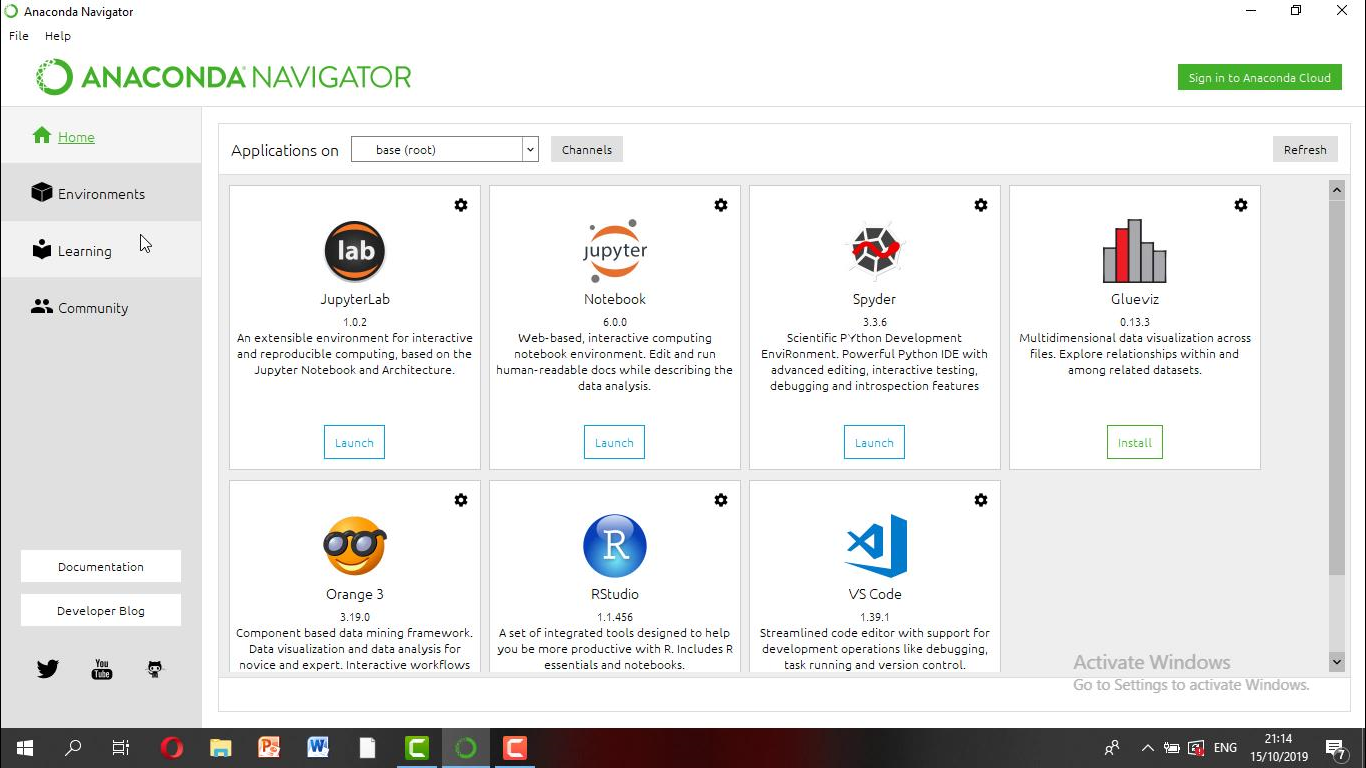
\includegraphics[scale=0.2]{gambar/17.png}
    \caption{}
    \label{fig:my_label}
\end{figure}
\item Setelah itu klik environments dan cari yang akan kita update
\begin{figure}[h]
    \centering
    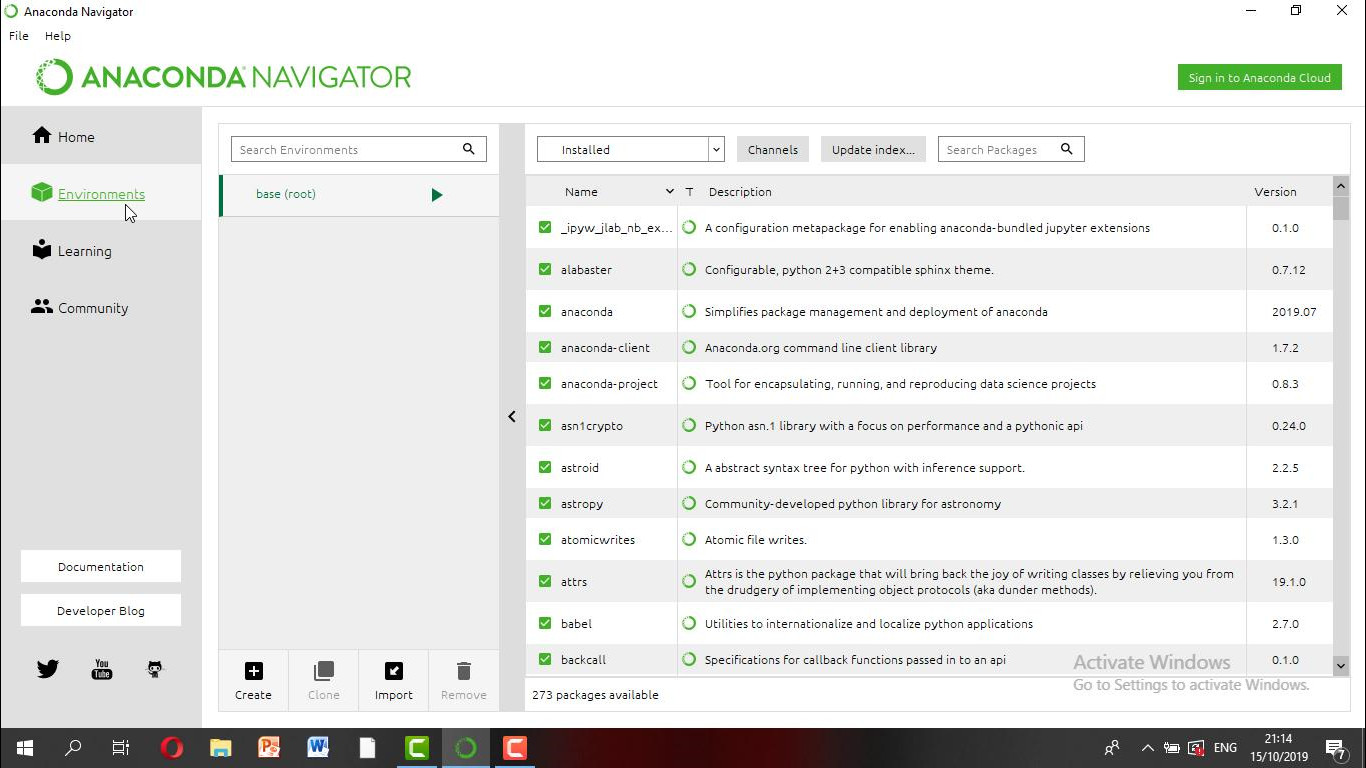
\includegraphics[scale=0.2]{gambar/18.png}
    \caption{}
    \label{fig:my_label}
\end{figure}
\item Lalu pilih spyder versi terbaru dari yang akan kita update
\begin{figure}[h]
    \centering
    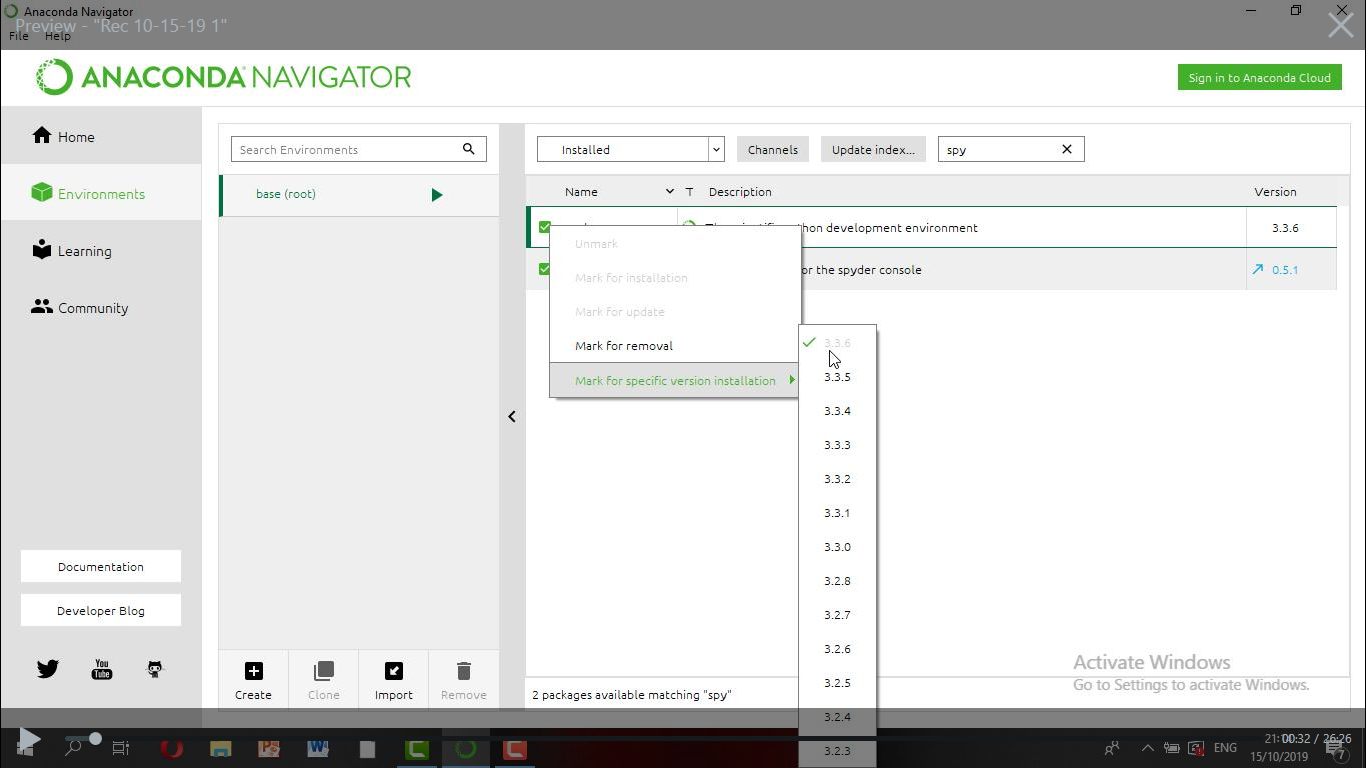
\includegraphics[scale=0.2]{gambar/19.png}
    \caption{}
    \label{fig:my_label}
\end{figure}
\item Begitu juga dengan anaconda yang akan kita update
\begin{figure}[h]
    \centering
    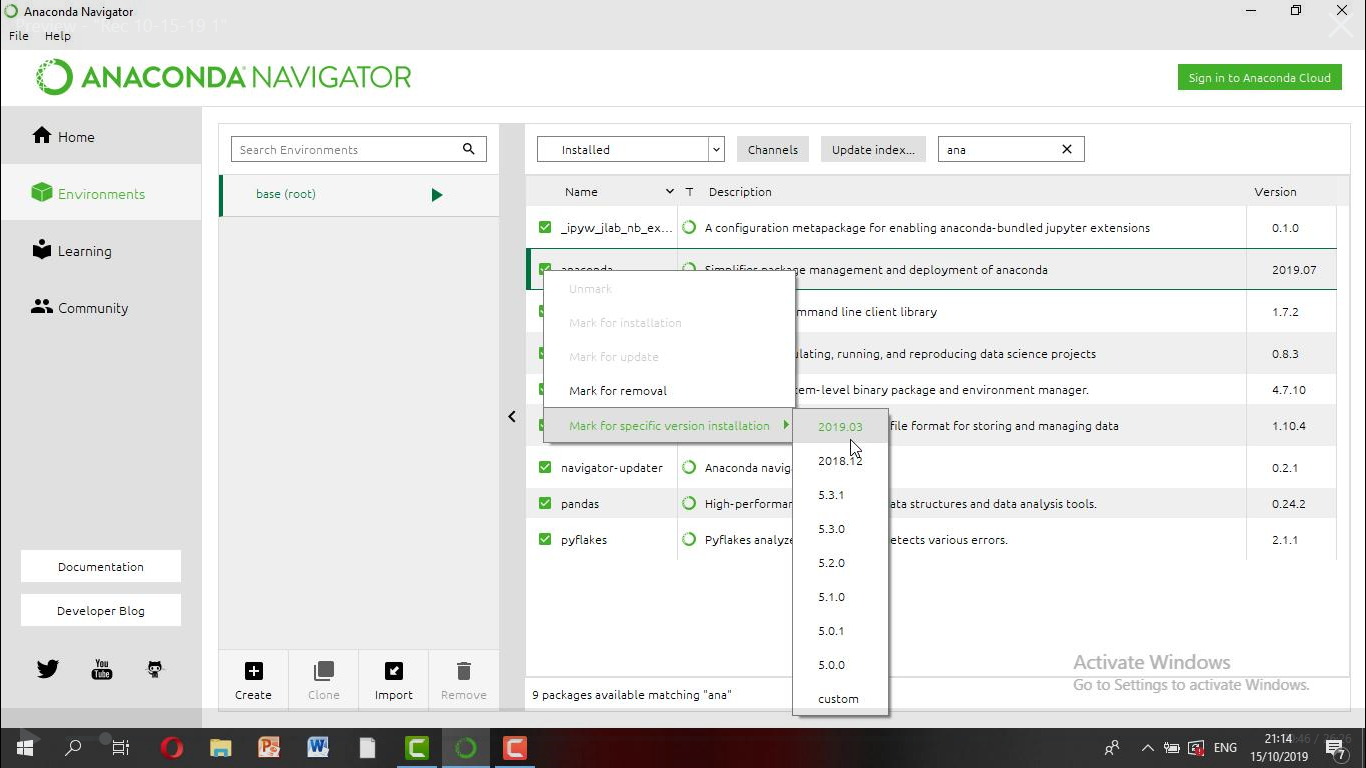
\includegraphics[scale=0.2]{gambar/20.png}
    \caption{}
    \label{fig:my_label}
\end{figure}
\item Setelah itu klik apply
\begin{figure}[h]
    \centering
    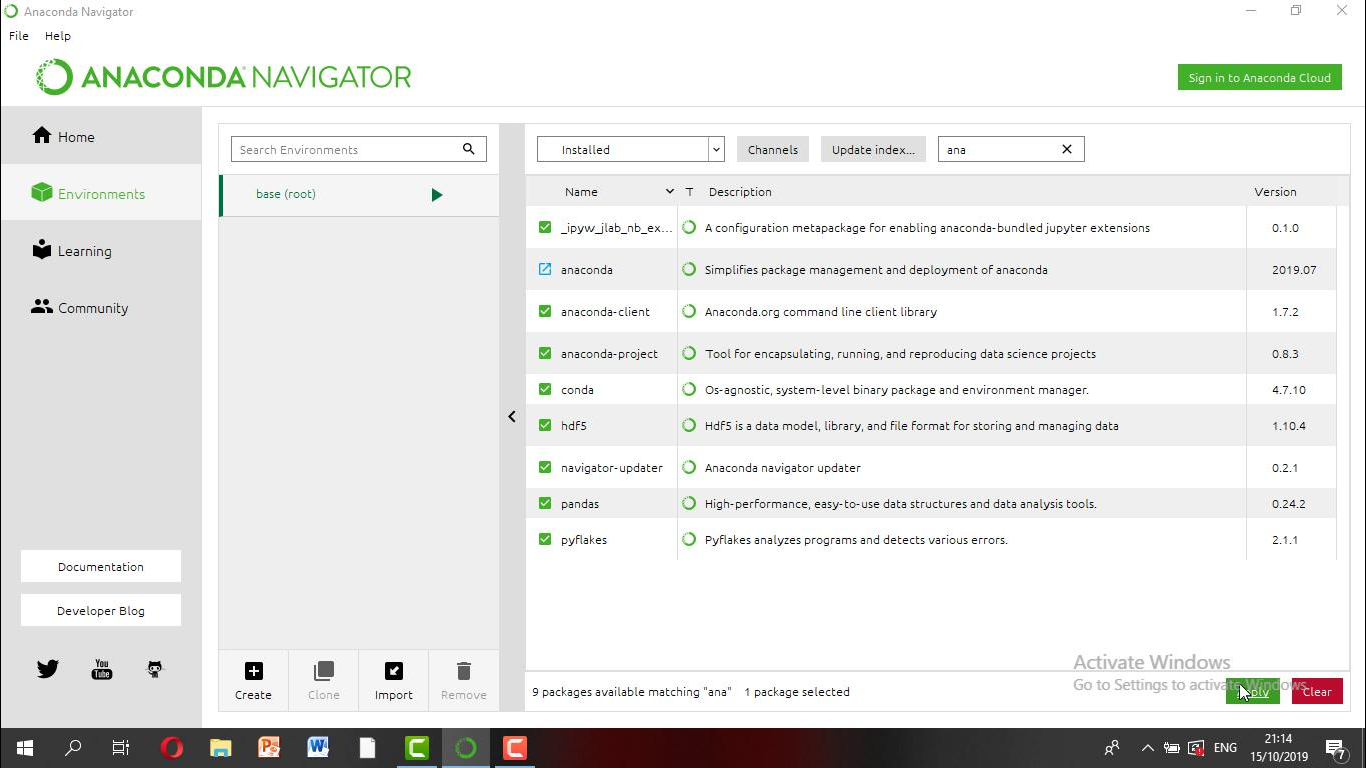
\includegraphics[scale=0.2]{gambar/21.png}
    \caption{}
    \label{fig:my_label}
\end{figure}
\item Dan tunggu sampai proses selesai
\begin{figure}[h]
    \centering
    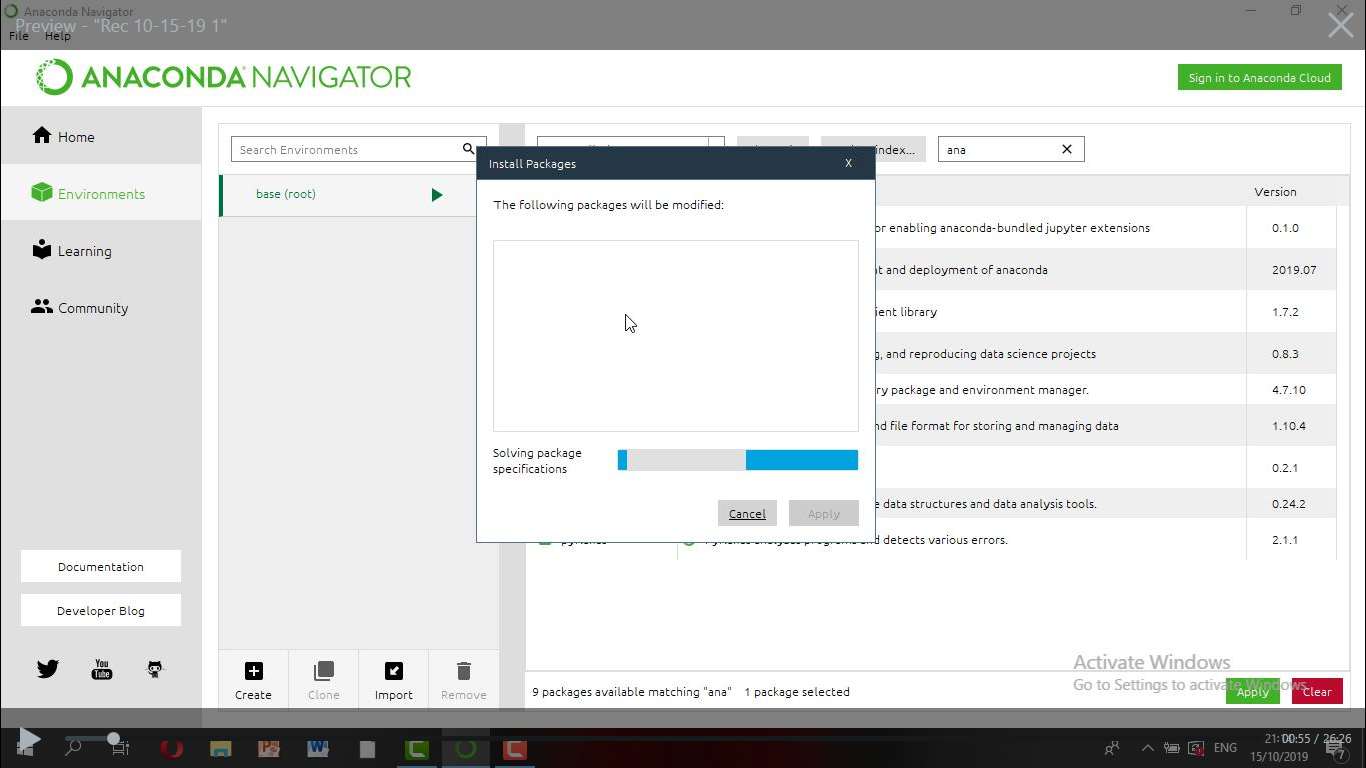
\includegraphics[scale=0.2]{gambar/22.png}
    \caption{}
    \label{fig:my_label}
\end{figure}
\item Jika sudah seperti tampilan dibawah ini, lalu klik apply lagi
\begin{figure}[h]
    \centering
    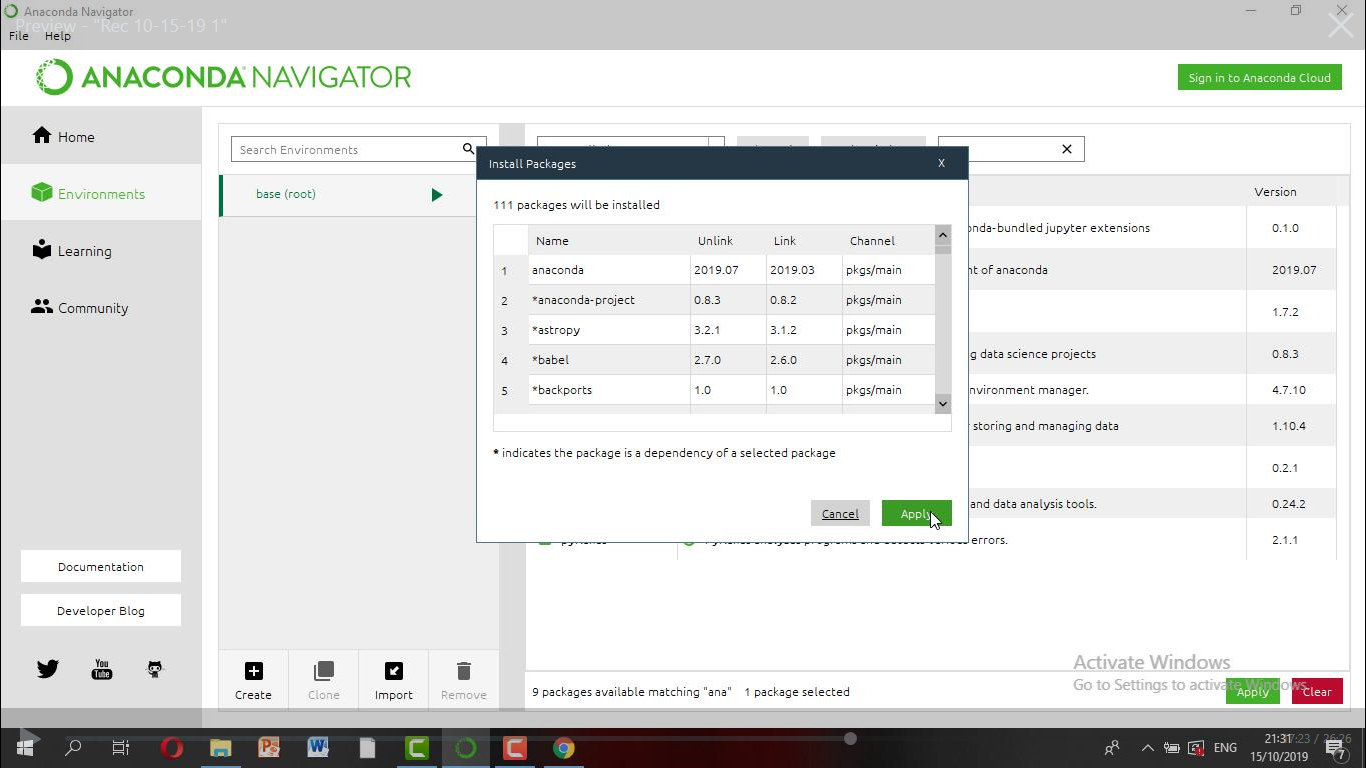
\includegraphics[scale=0.2]{gambar/23.png}
    \caption{}
    \label{fig:my_label}
\end{figure}
\item Kemudian tunggu sampai proses selesai
\begin{figure}[h]
    \centering
    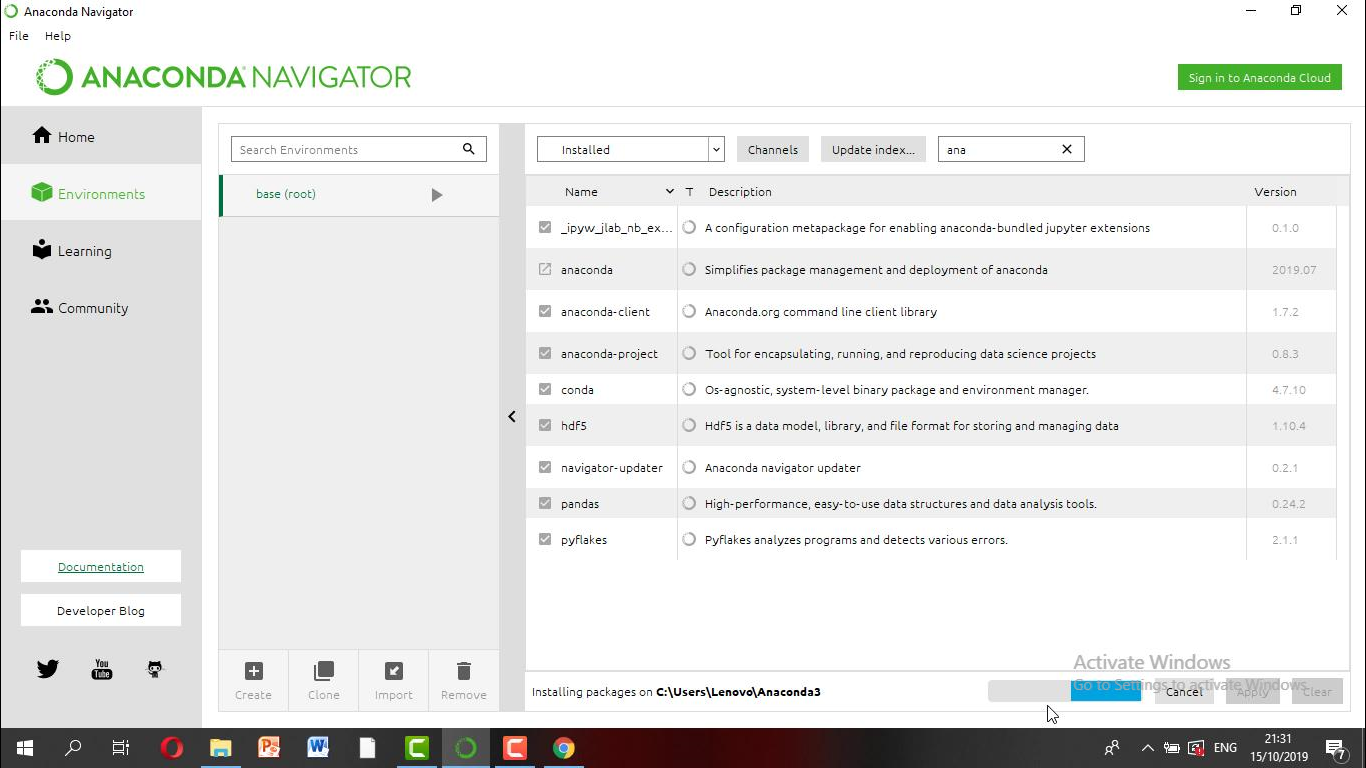
\includegraphics[scale=0.2]{gambar/24.png}
    \caption{}
    \label{fig:my_label}
\end{figure}
\section*{CARA SETTING ENVIRONMENT}
\begin{enumerate}
\item  Buka file exploler, setelah itu klik kanan di this pc, pilih properties
\begin{figure}[h]
    \centering
    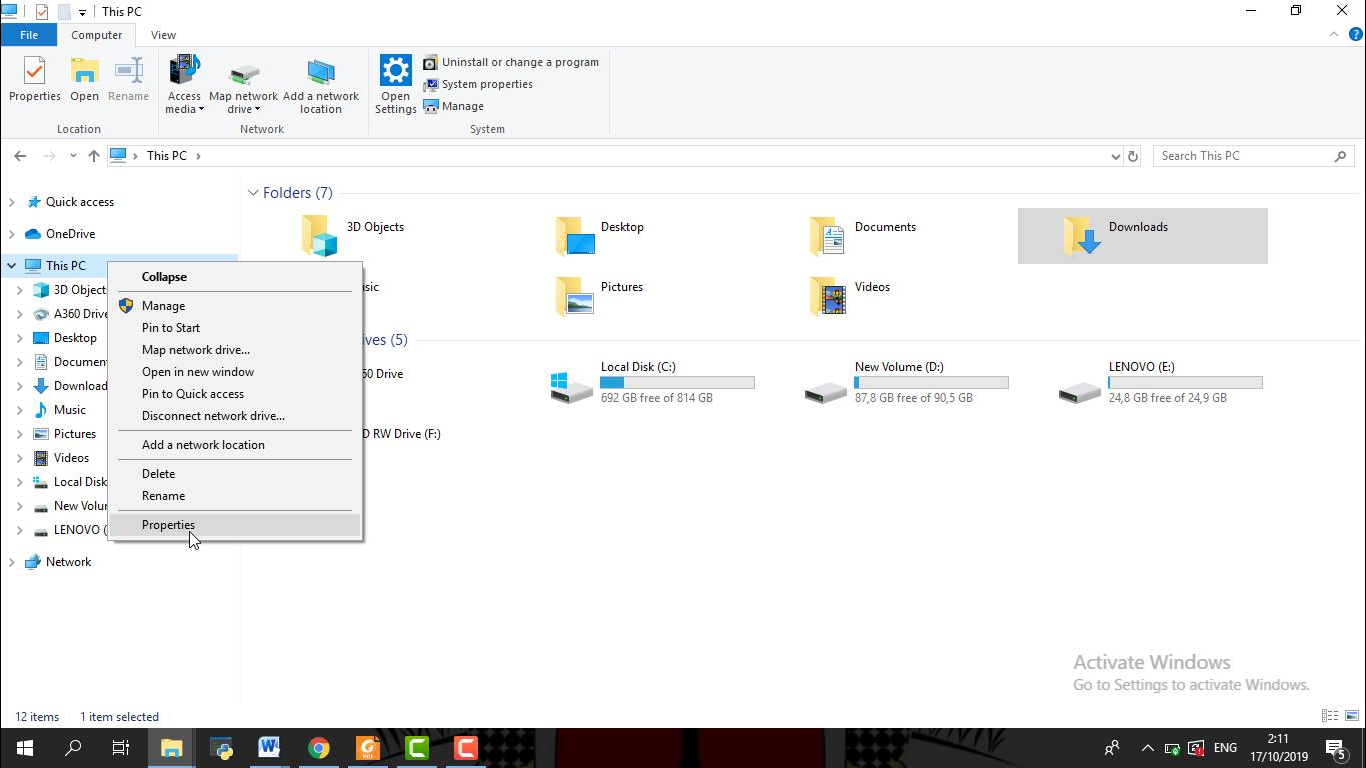
\includegraphics[scale=0.2]{gambar/25.png}
    \caption{}
    \label{fig:my_label}
\end{figure}
\item Lalu buka advance system settings
\begin{figure}[h]
    \centering
    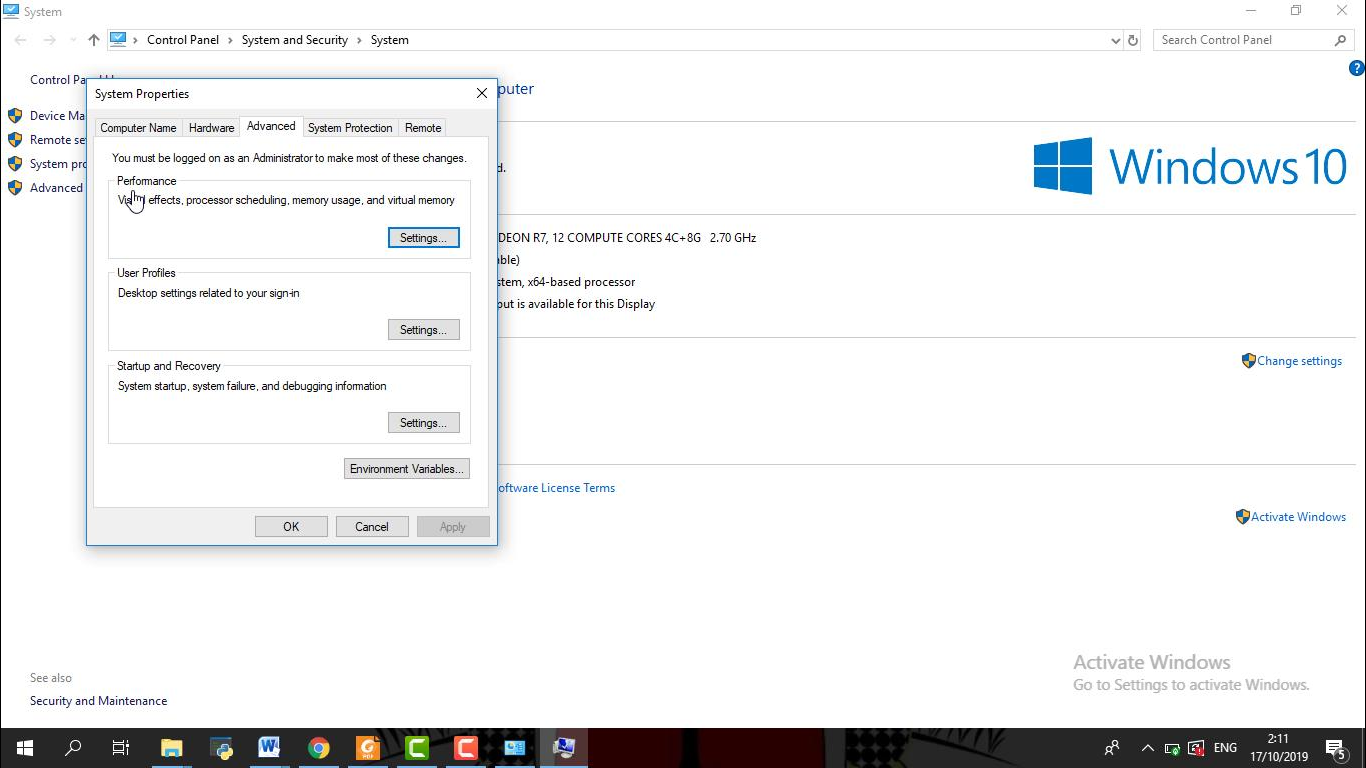
\includegraphics[scale=0.2]{gambar/26.png}
    \caption{}
    \label{fig:my_label}
\end{figure}
\item Setelah itu klik environment variables
\begin{figure}[h]
    \centering
    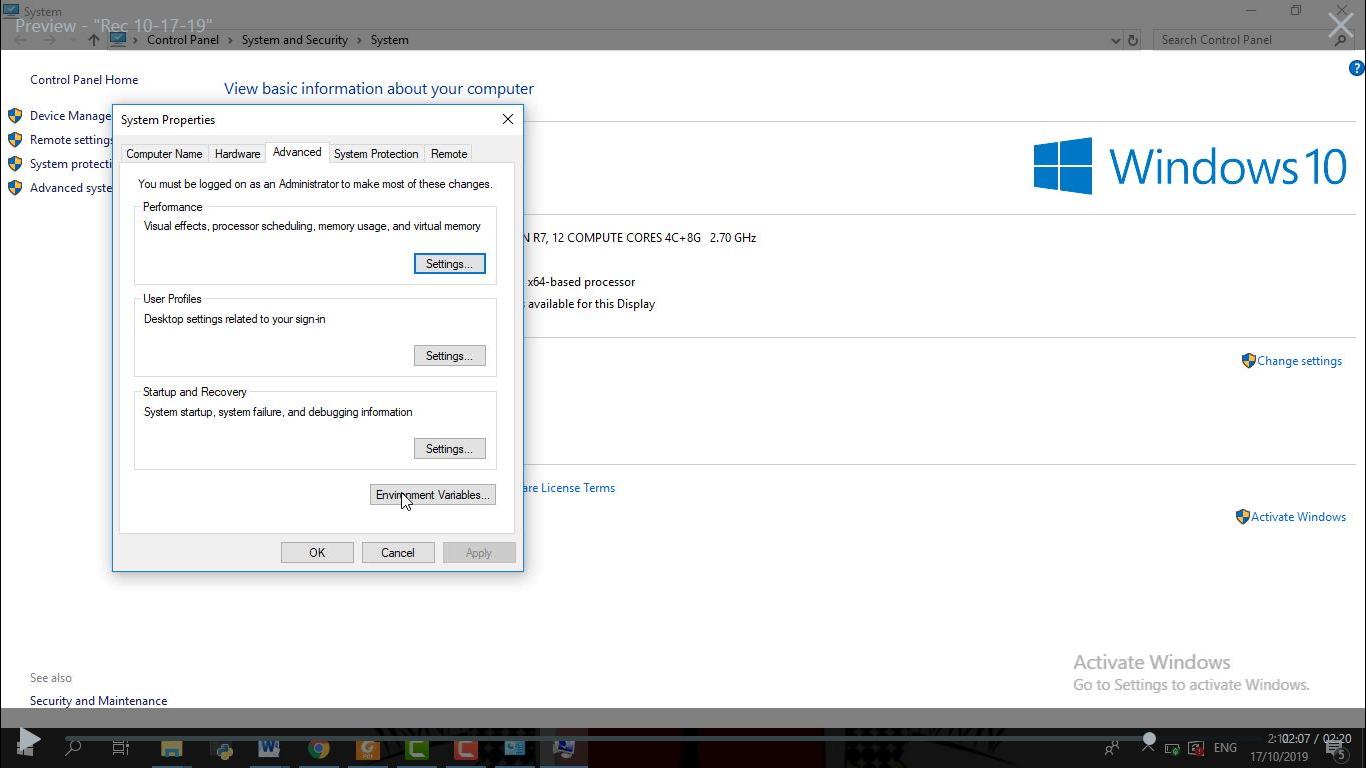
\includegraphics[scale=0.2]{gambar/27.png}
    \caption{}
    \label{fig:my_label}
\end{figure}
\item Jika ingin menggaturnya maka pilih edit
\begin{figure}[h]
    \centering
    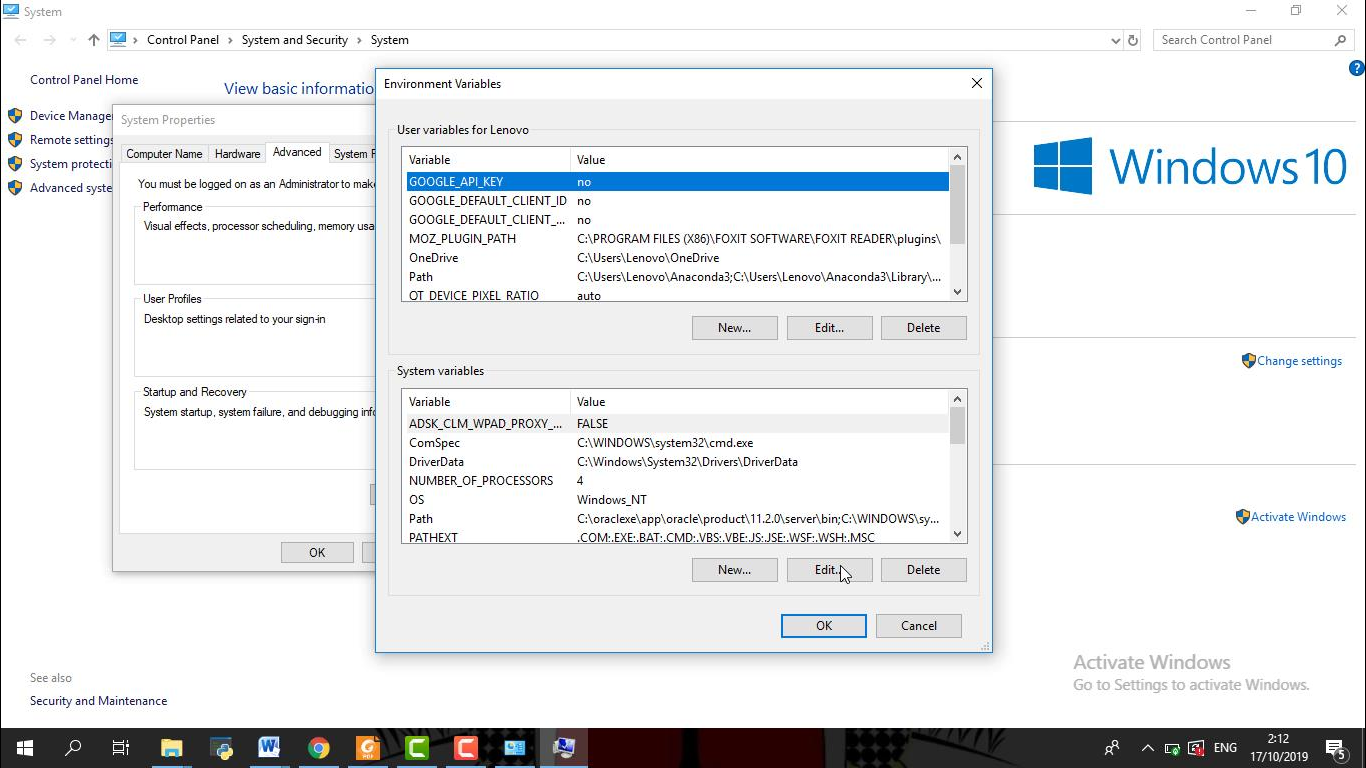
\includegraphics[scale=0.2]{gambar/28.png}
    \caption{}
    \label{fig:my_label}
\end{figure}
\section*{Mencoba Entrepreter/cli melalui Terminal atau cmd
windows}
\begin{enumerate}
\item  Pertama buka cmd
\begin{figure}[h]
    \centering
    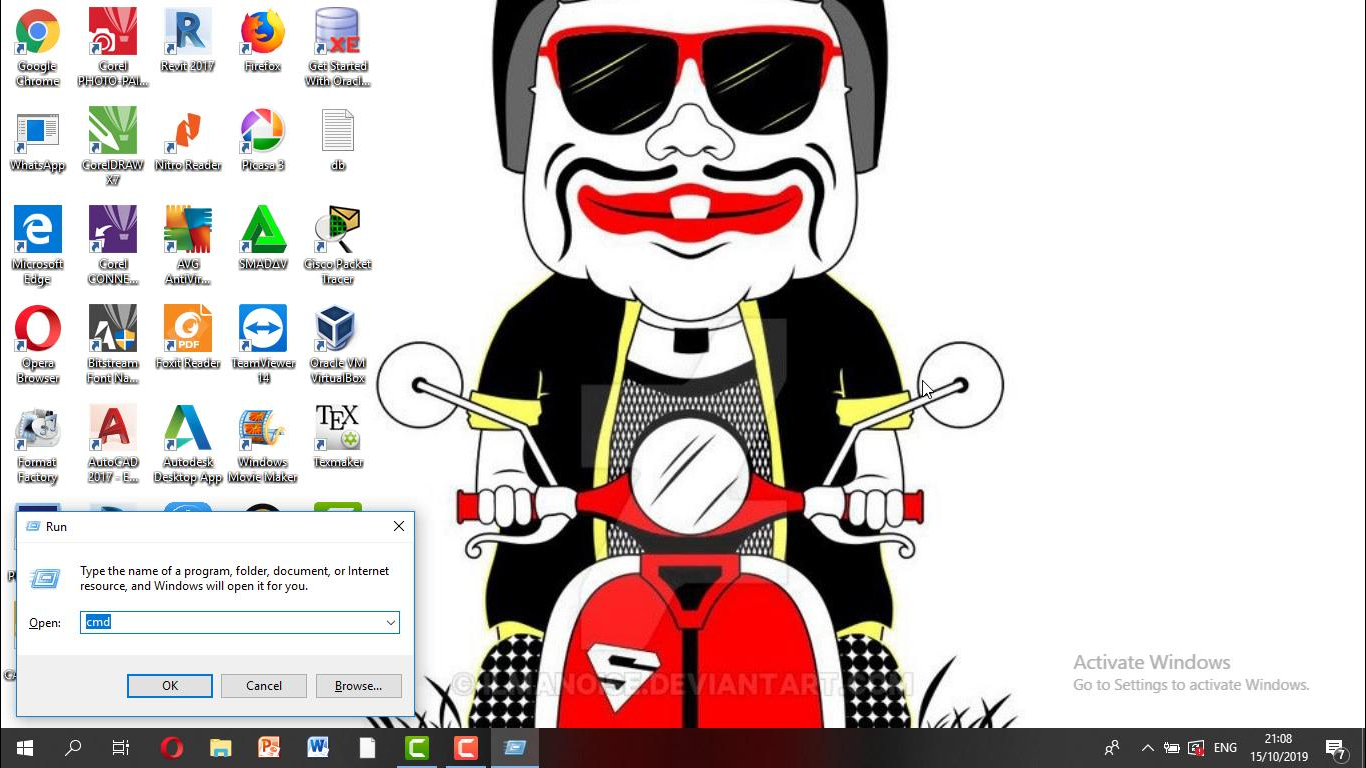
\includegraphics[scale=0.2]{gambar/29.png}
    \caption{}
    \label{fig:my_label}
\end{figure}
\item  Setelah itu ketik python, kemudian ketik print("helo world")
\begin{figure}[h]
    \centering
    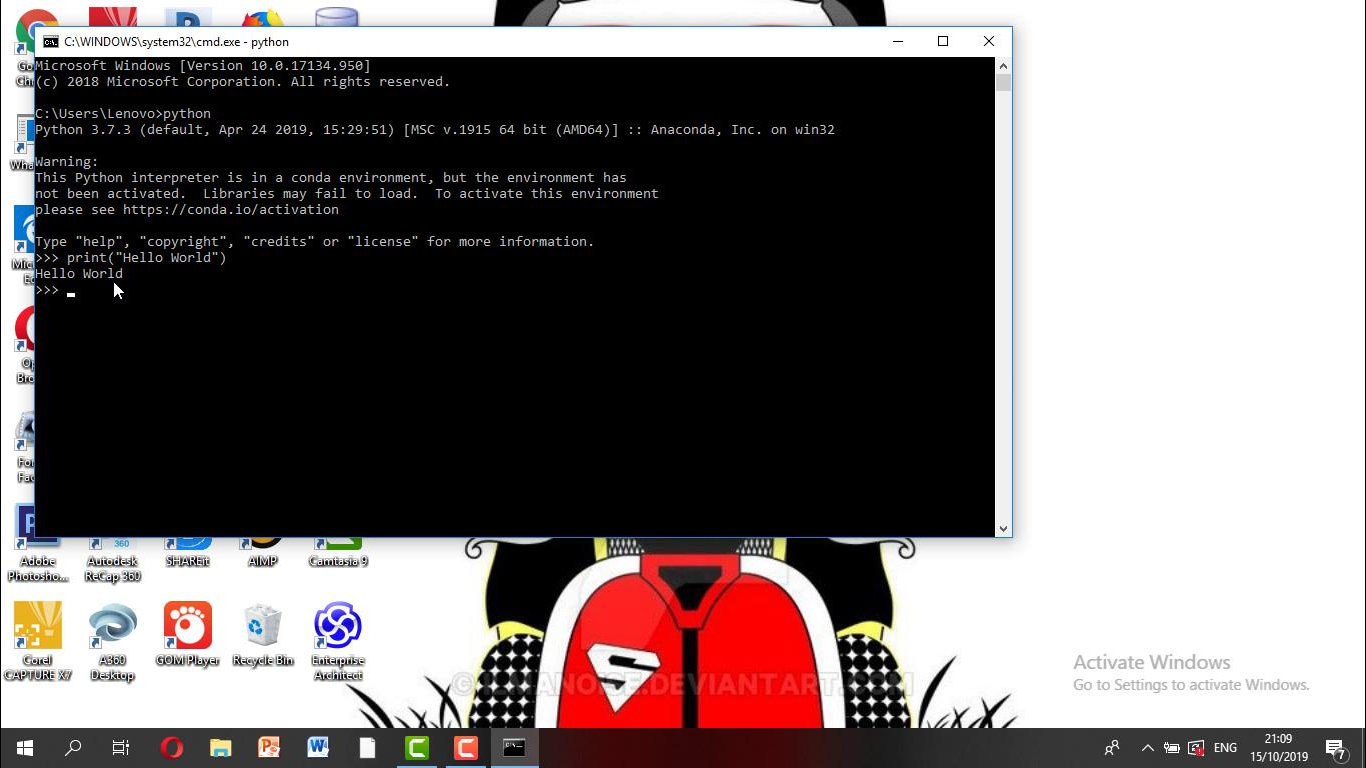
\includegraphics[scale=0.2]{gambar/30.png}
    \caption{}
    \label{fig:my_label}
\end{figure}
\section*{Cara menjalankan Script hello word di spyder serta penggunaan variabel exploler di spyder}
\begin{enumerate}
\item  Pertama buka spydernya
\begin{figure}[h]
    \centering
    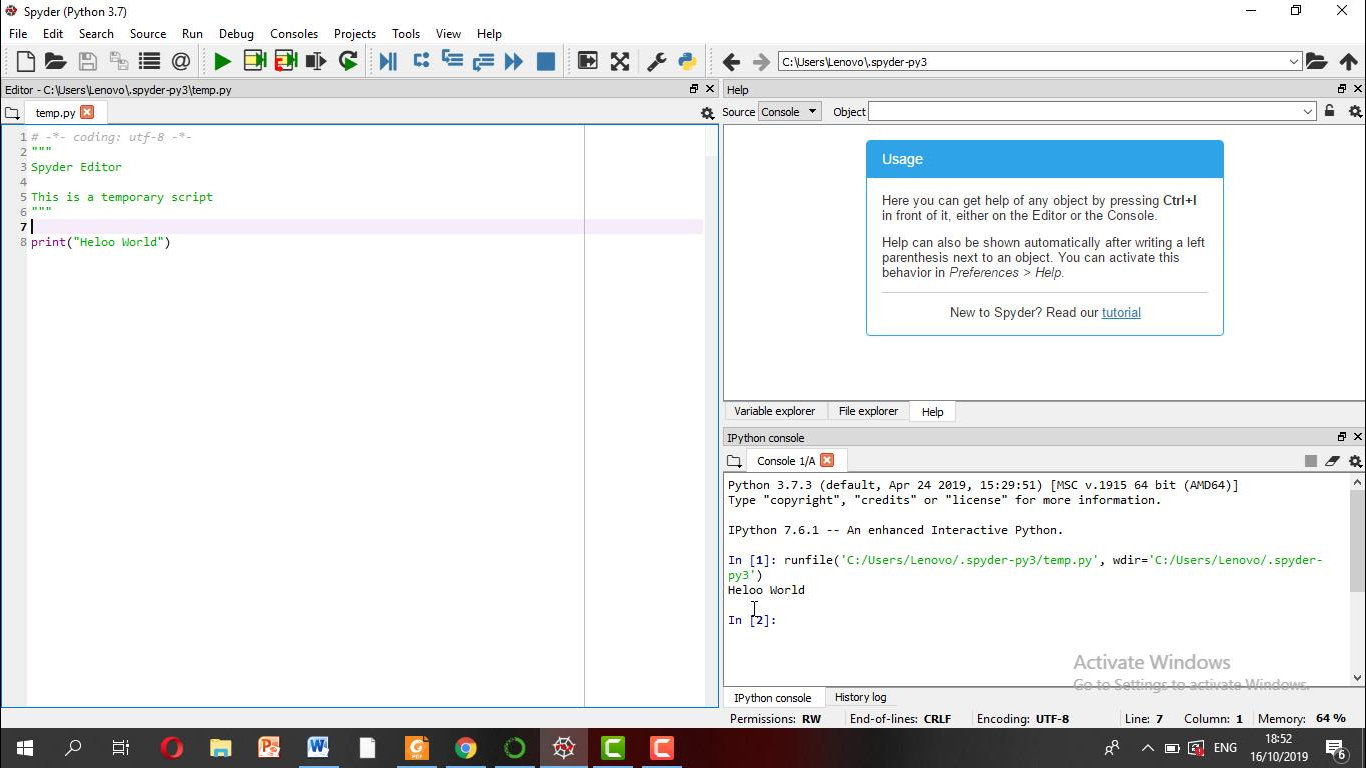
\includegraphics[scale=0.2]{gambar/31.png}
    \caption{}
    \label{fig:my_label}
\end{figure}
\item  Setelah itu ketik scriptnya("helo world")
\begin{figure}[h]
    \centering
    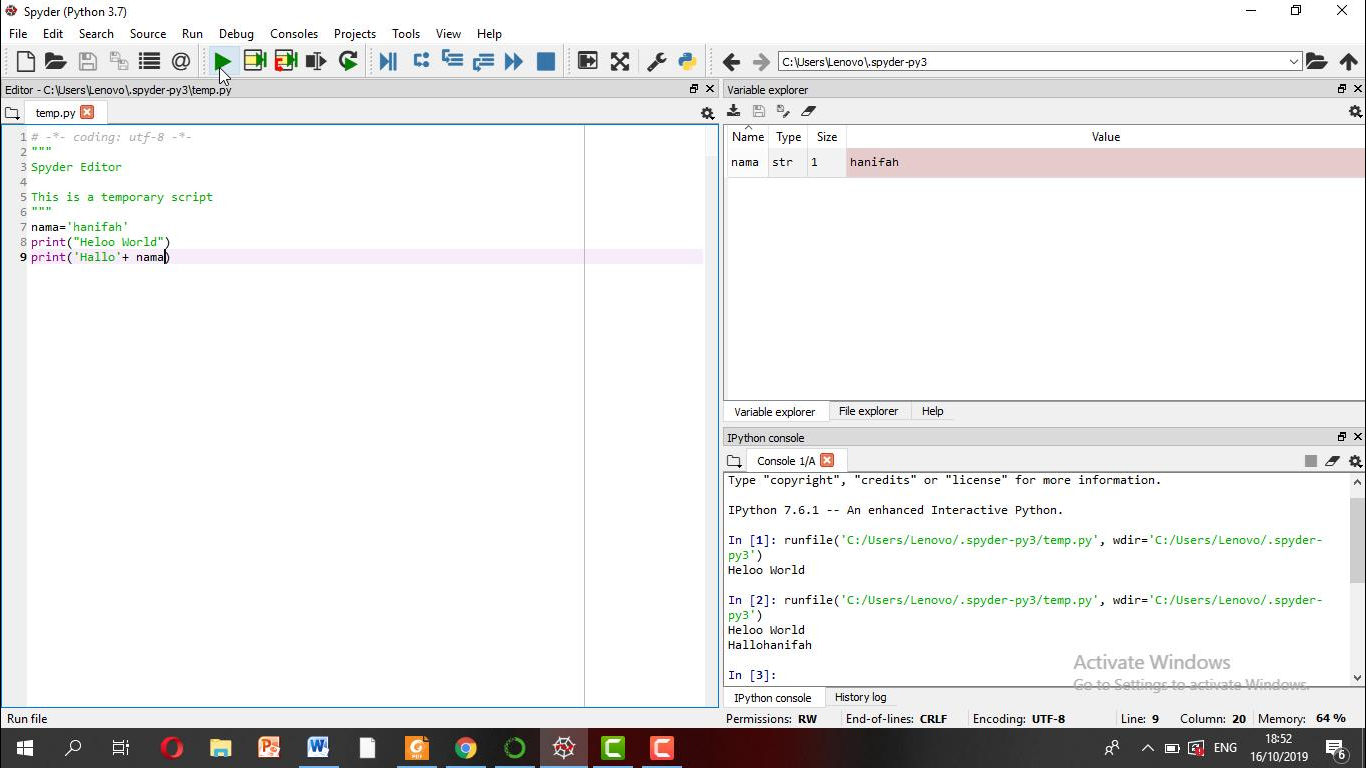
\includegraphics[scale=0.2]{gambar/32.png}
    \caption{}
    \label{fig:my_label}
\end{figure}
\item  Hasilnya berupa nama,type, serta value dari variabel
\begin{figure}[h]
    \centering
    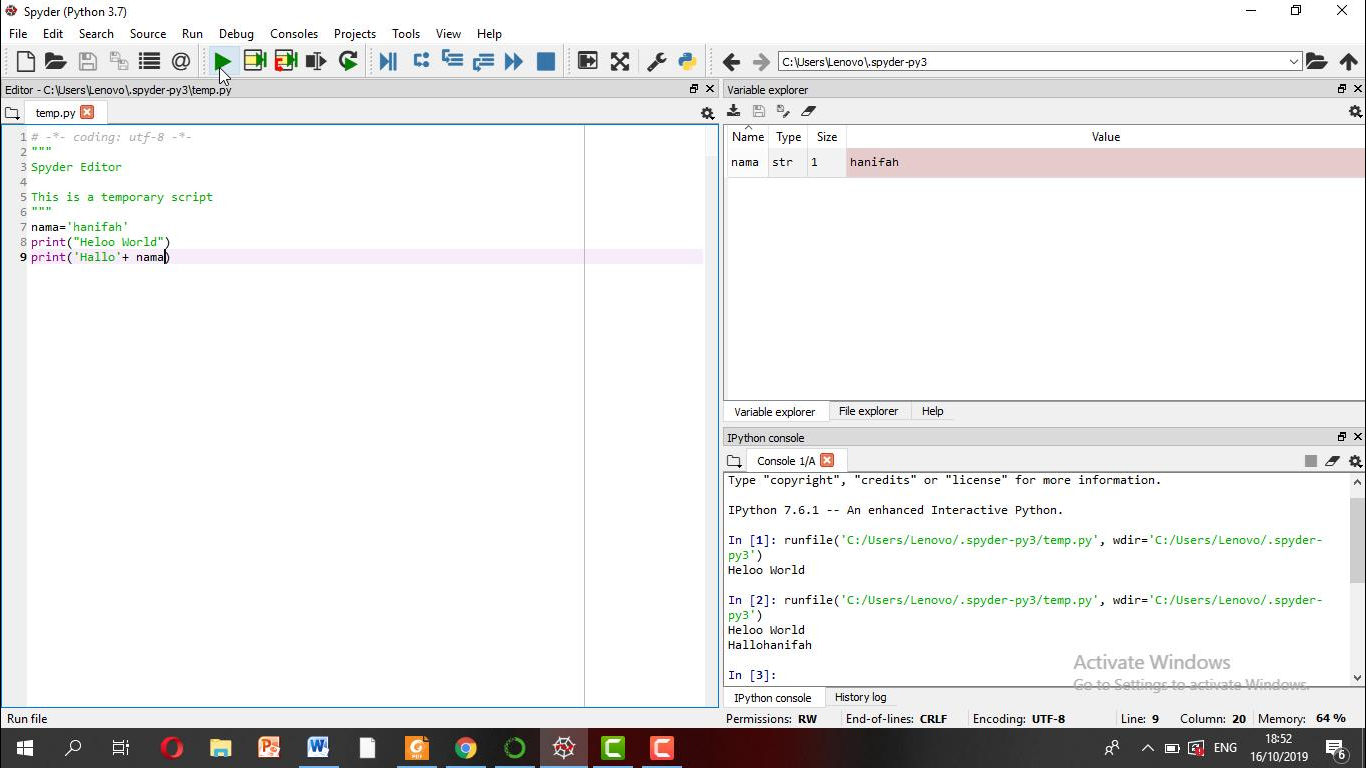
\includegraphics[scale=0.2]{gambar/34.png}
    \caption{}
    \label{fig:my_label}
\end{figure}
\section*{ Cara menjalankan Script otomatis login aplikasi akademik dengan library selenium dan inputan user}
\begin{enumerate}
\item  Pertama buka spydernya, lalu ketik scriptnya
\begin{figure}[h]
    \centering
    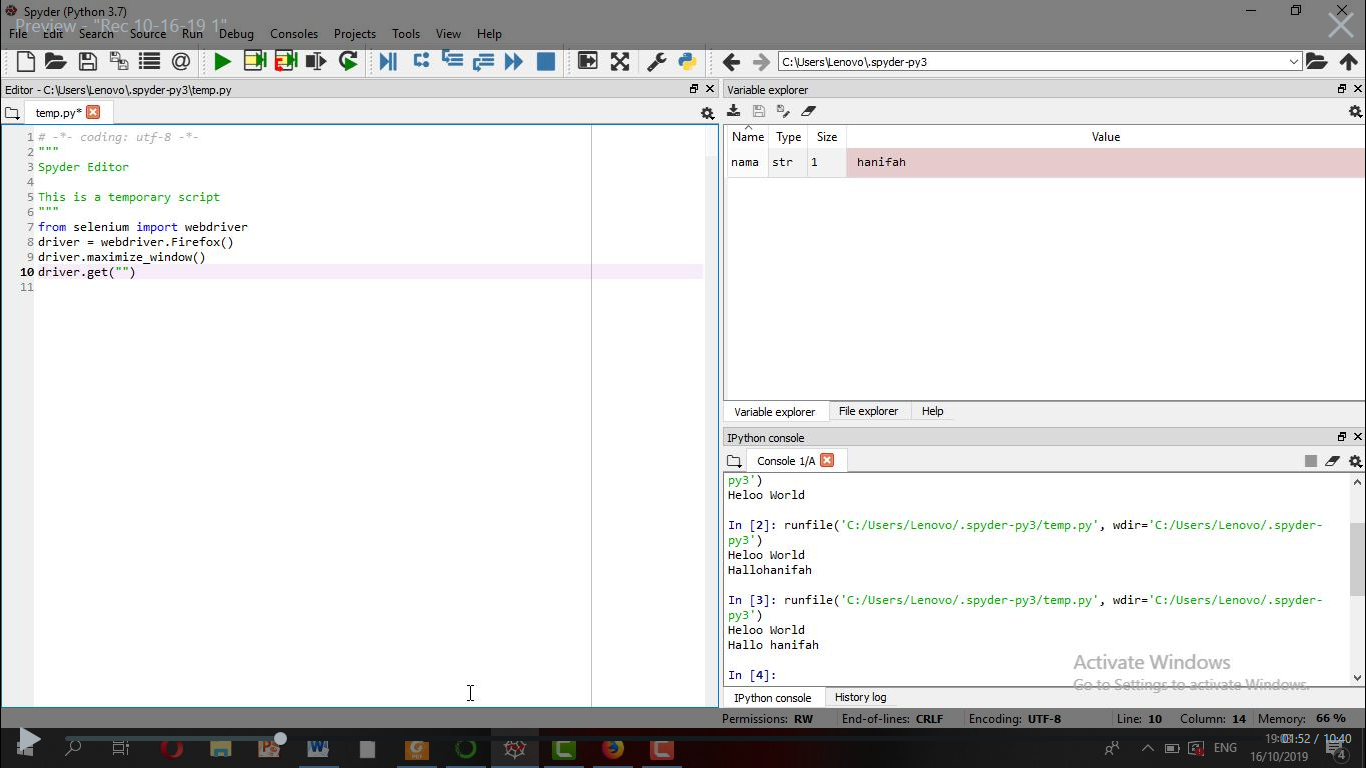
\includegraphics[scale=0.2]{gambar/36.png}
    \caption{}
    \label{fig:my_label}
\end{figure}
\item  Setelah itu, buka web siap.poltekpos serta copy alamat webnya.
\begin{figure}[h]
    \centering
    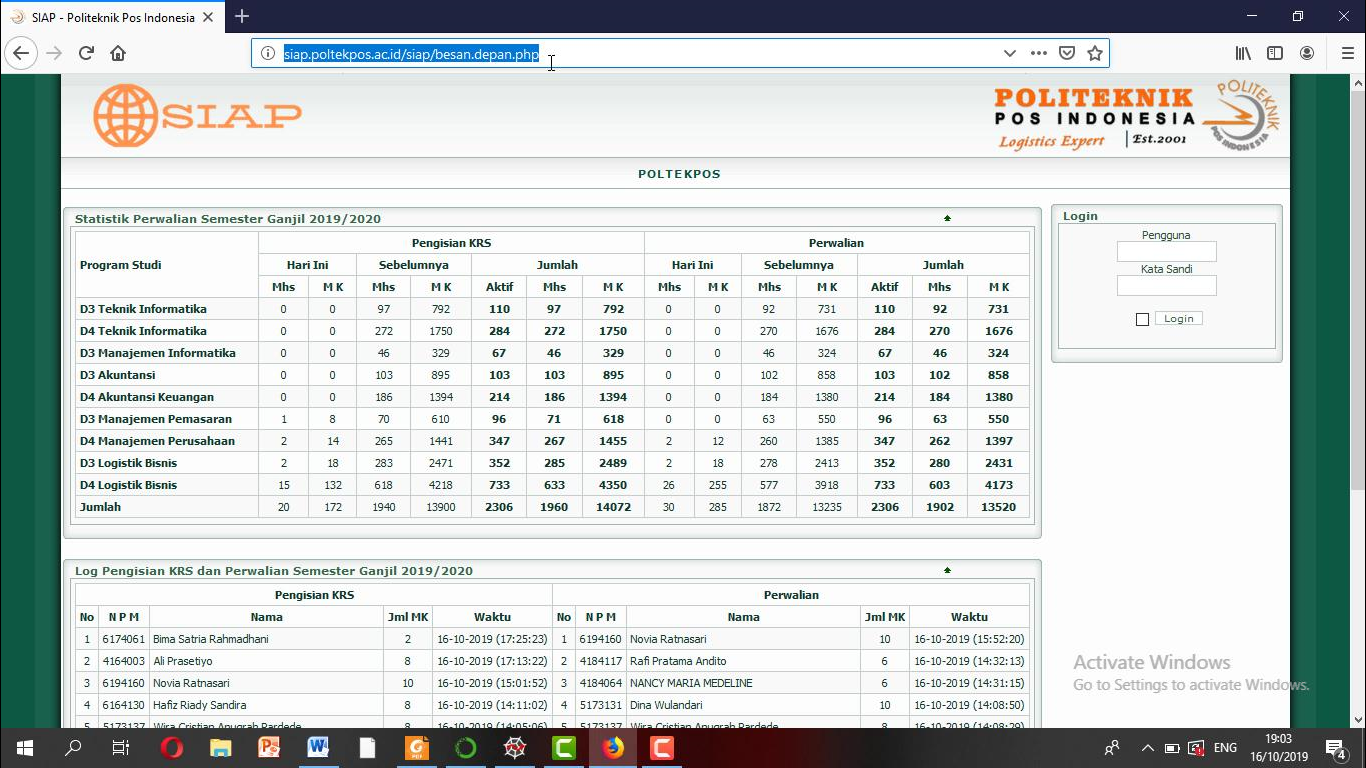
\includegraphics[scale=0.2]{gambar/37.png}
    \caption{}
    \label{fig:my_label}
\end{figure}
\item  Kemudian,copy alamat webnya kedalam script di spyder
\begin{figure}[h]
    \centering
    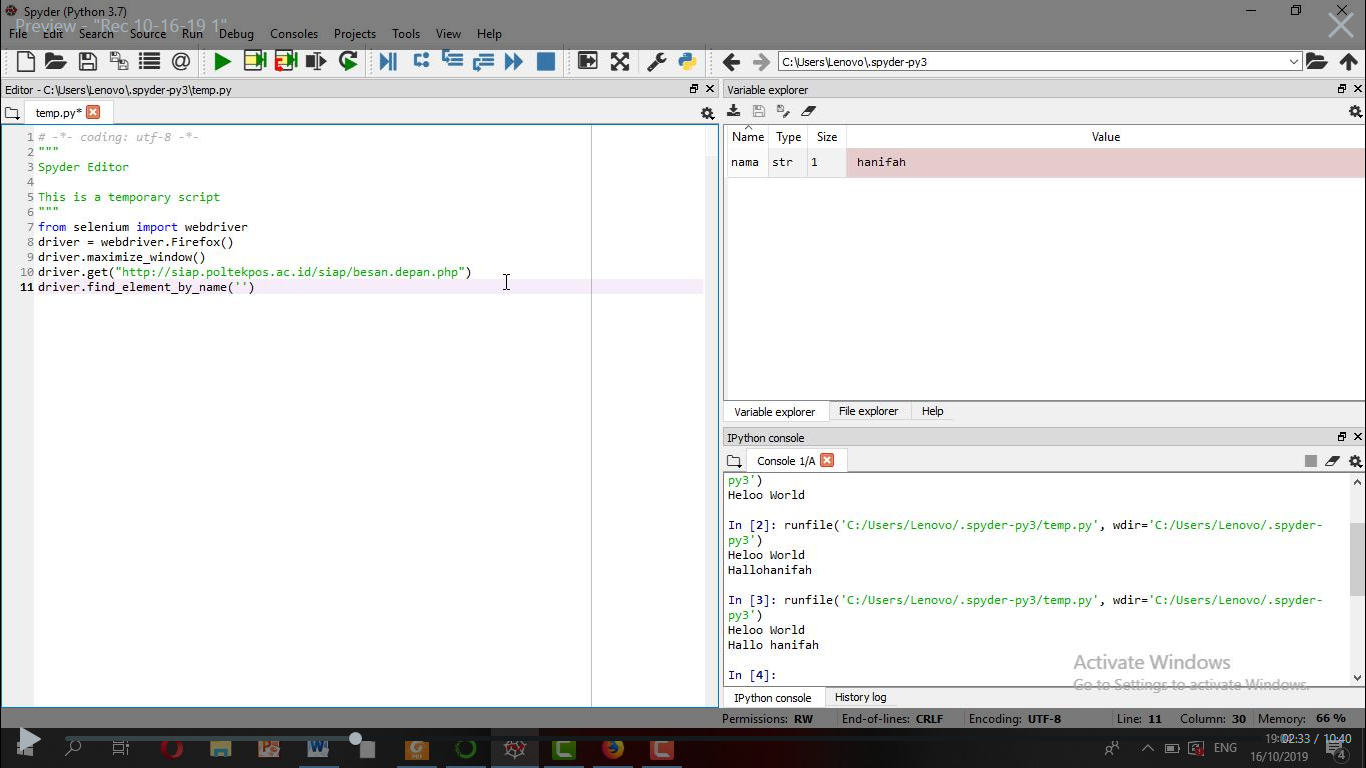
\includegraphics[scale=0.2]{gambar/38.png}
    \caption{}
    \label{fig:my_label}
\end{figure}
\item  Setelah itu,klik tombol inspect element pada siap.poltekposnya
\begin{figure}[h]
    \centering
    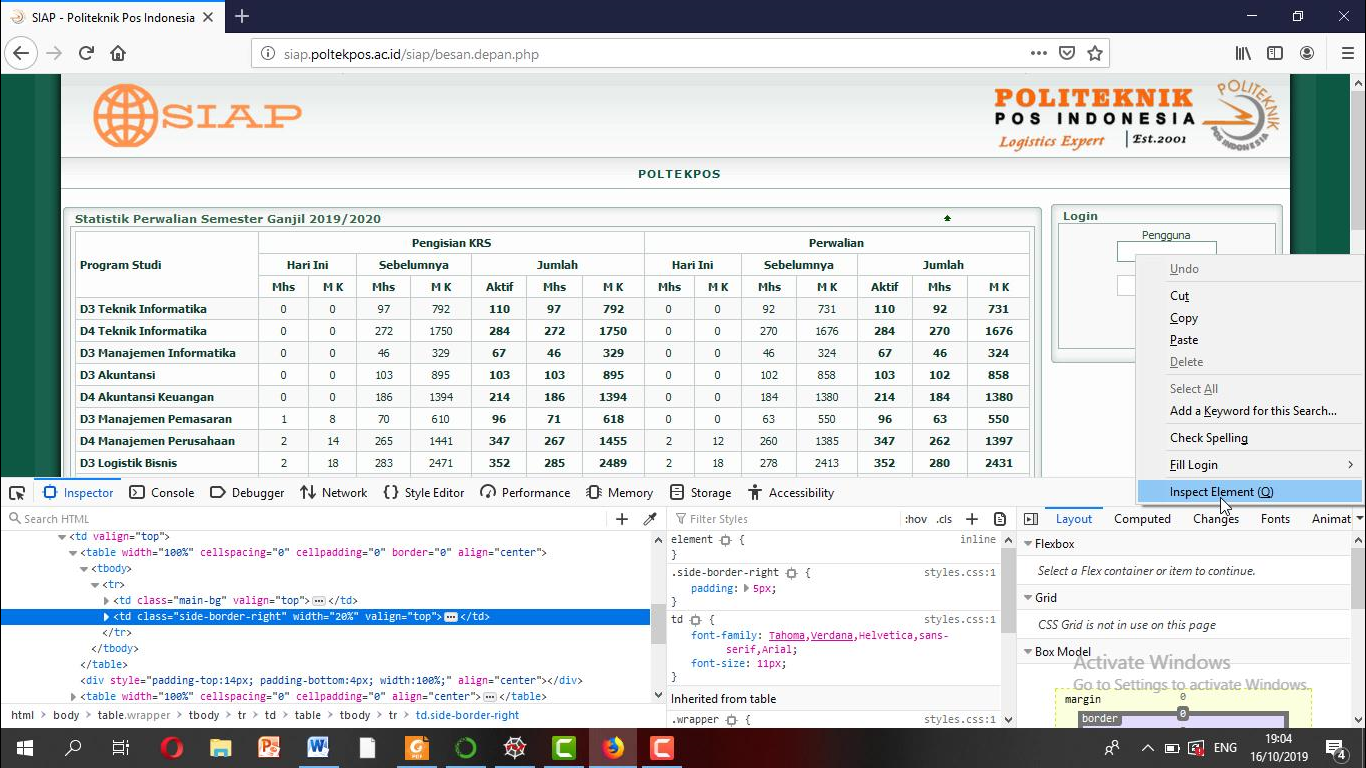
\includegraphics[scale=0.2]{gambar/39.png}
    \caption{}
    \label{fig:my_label}
\end{figure}
\item   karena seleniumnya belum diinstall,maka install dulu di cmd
\begin{figure}[h]
    \centering
    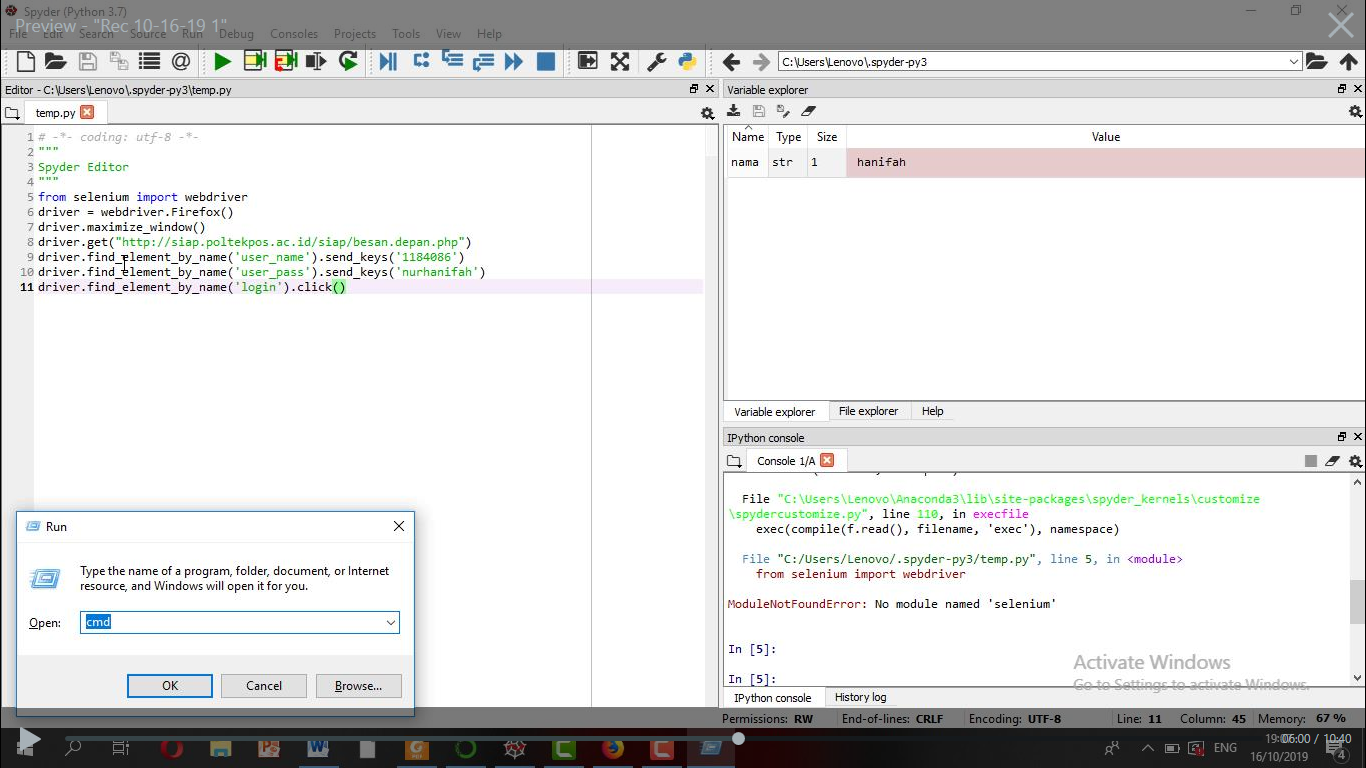
\includegraphics[scale=0.2]{gambar/40.png}
    \caption{}
    \label{fig:my_label}
\end{figure}
\item  Selanjutnya ketik pip install selenium pada cmd
\begin{figure}[h]
    \centering
    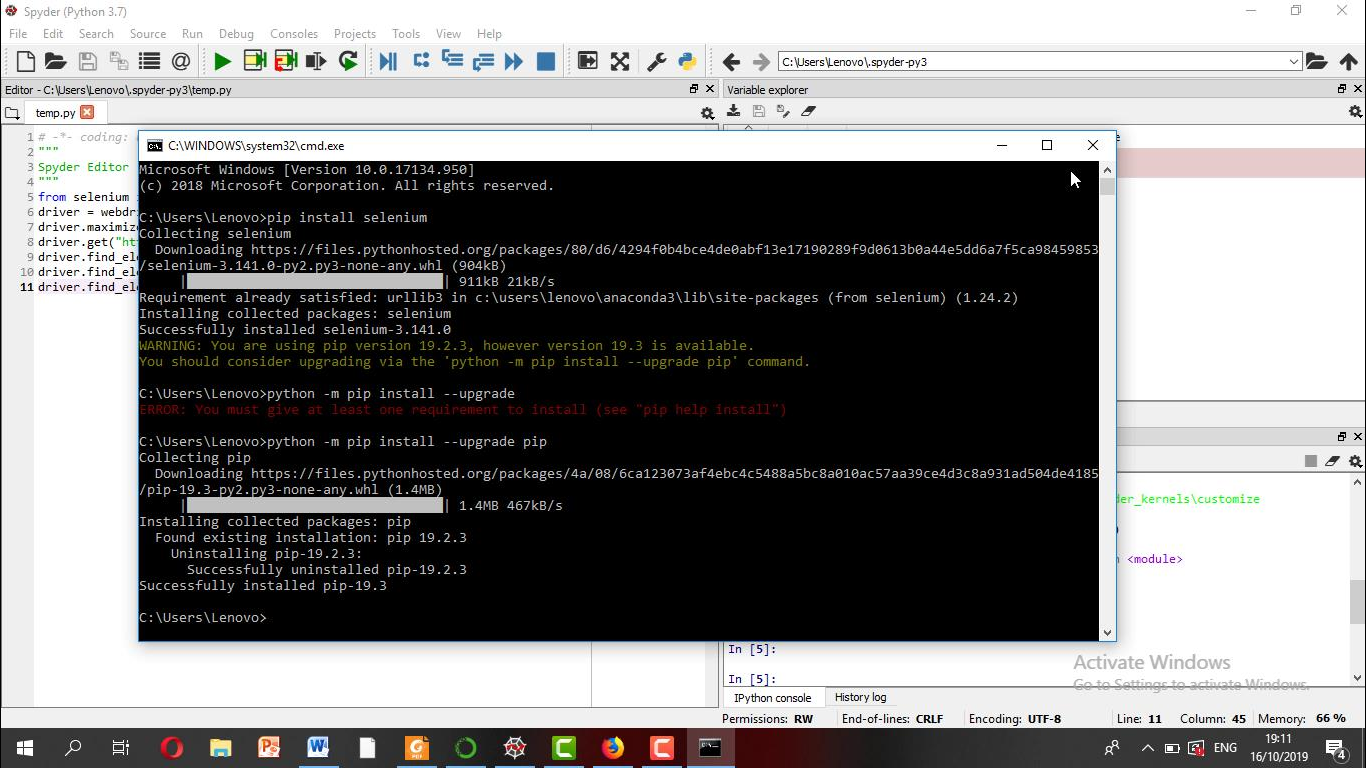
\includegraphics[scale=0.2]{gambar/41.png}
    \caption{}
    \label{fig:my_label}
\end{figure}
\item  Selanjutnya ketik script lagi pada spyder
\begin{figure}[h]
    \centering
    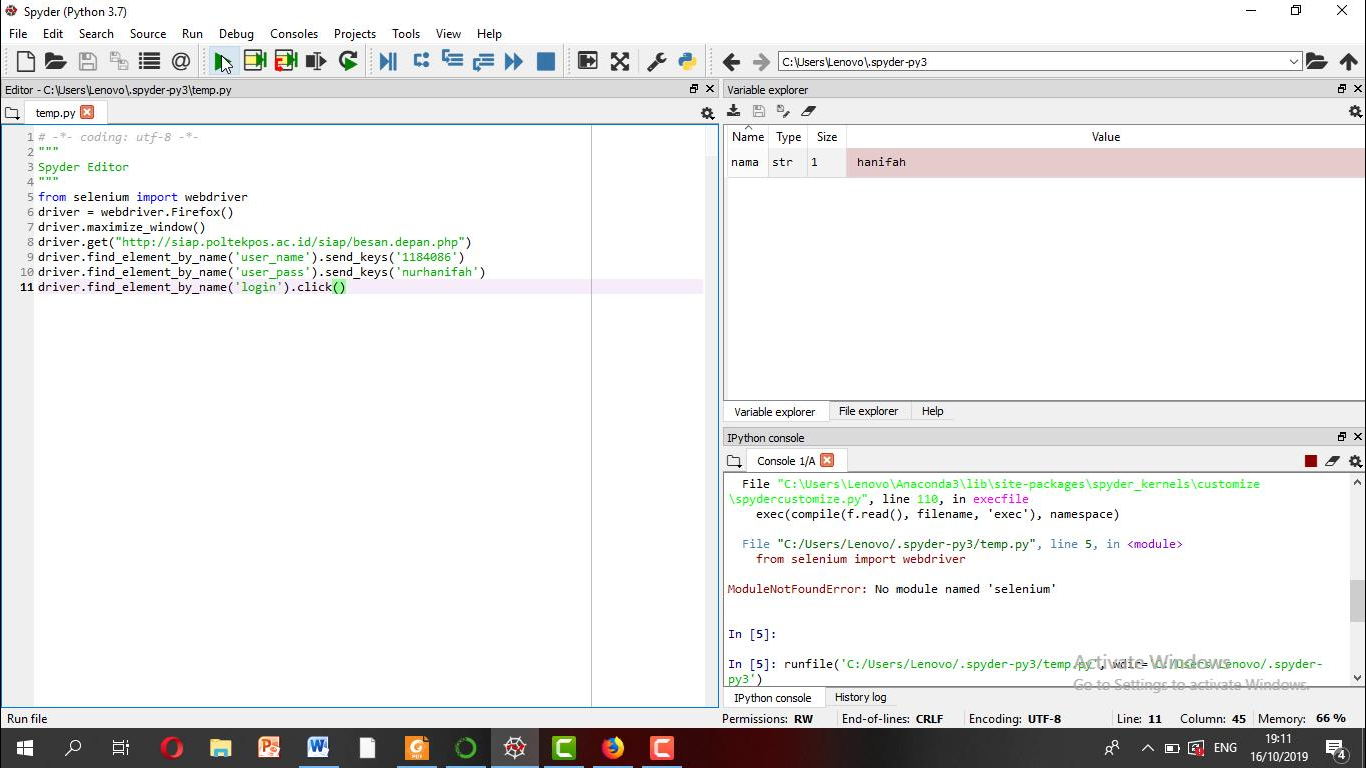
\includegraphics[scale=0.2]{gambar/42.png}
    \caption{}
    \label{fig:my_label}
\end{figure}
\item  Setelah itu buka aplikasi siap.poltekpos lagi
\begin{figure}[h]
    \centering
    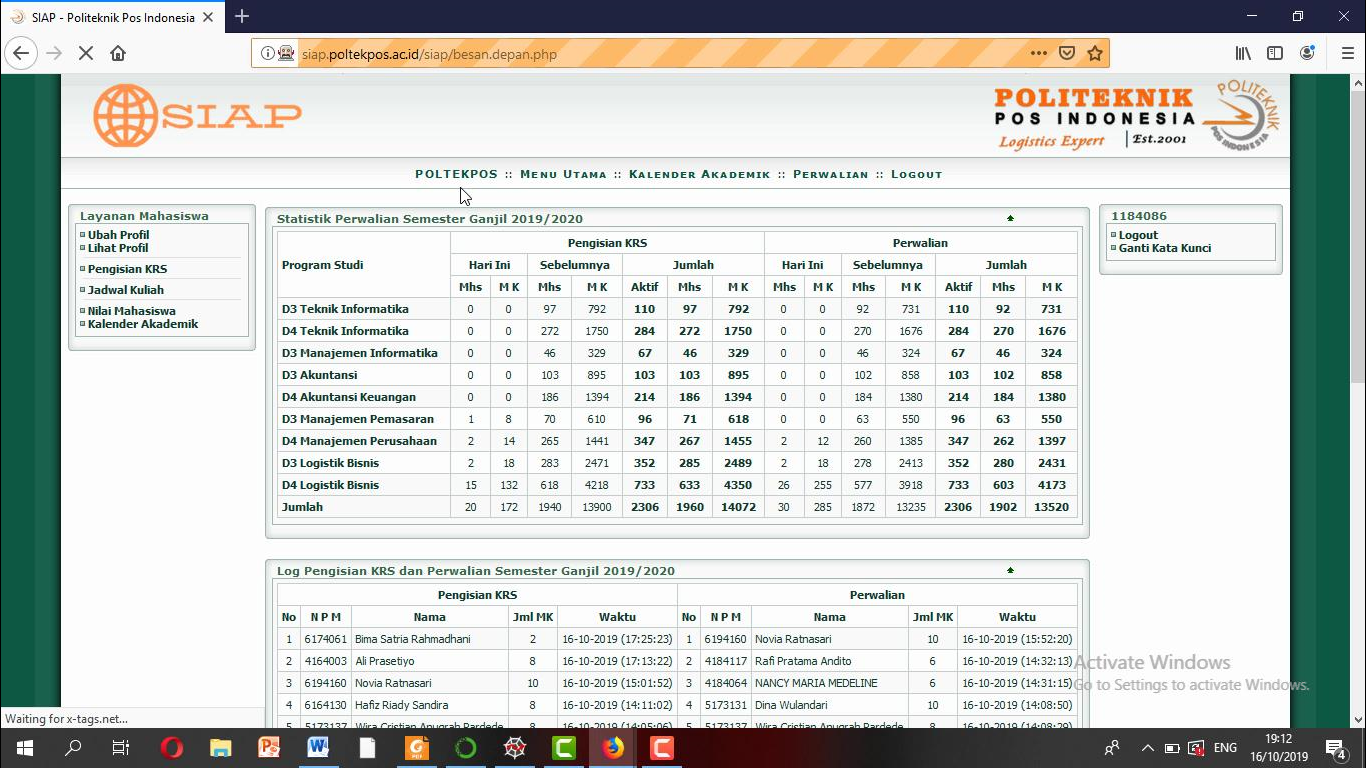
\includegraphics[scale=0.2]{gambar/43.png}
    \caption{}
    \label{fig:my_label}
\end{figure}
\section*{\textit{IDENTASI}}
\par
\textit{Penjelasan Identasi} yaitu dalam bahasa pemprograman python merupakan penulisan yang sedikit menjorok ke kanan, Identasi ini sangatlah mempengaruhi hasil eksekusi pada pemprograman ini.Identasi ini pada bahasa pemprograman python digunakan sebagai penanda blok program yang bertujuan dapat mempermudah membaca script yang telah dibuat.
Jenis-Jenis eror identasi:
Pada Python Identasi ini sangat mempengaruhi hasil eksekusi, karena identasi sendiri merupakan blok pemprograman. Kesalahan yang sering terjadi contohnya yaitu lupa identasi, identasi yang berbeda, lupa tanda kurang, dan lain sebagainya.
Cara membaca erorrnya yaitu jika terdapat tanda warning maka script kita terjadi erorr, maka dari itu cara menangganinya yaitu dengan memperhatikan warning kesalahan yang muncul pada jendela python setelah itu baru diperbiki kesalahn yang terjadi.
\par
\begin{figure}[h]
    \centering
    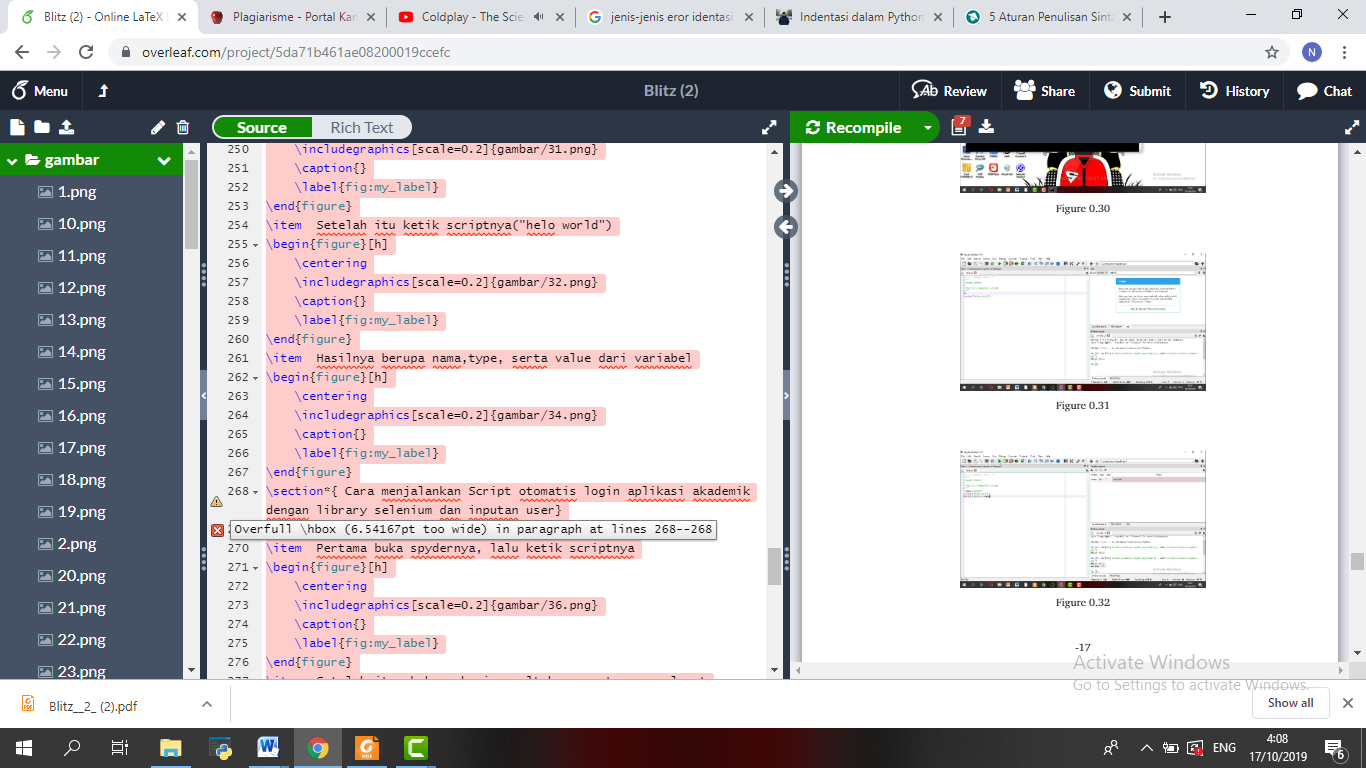
\includegraphics[scale=0.2]{gambar/44.png}
    \caption{contoh error identasi}
    \label{fig:my_label}
\end{figure}
\end{enumerate}
\end{enumerate}
\end{enumerate}
\end{enumerate}
\end{enumerate}
\end{enumerate}

